\IfFileExists{IEEEtran.cls}{%
\documentclass[conference,compsoc]{IEEEtran}
}{%
\documentclass[10pt,twocolumn]{article}
\newcommand{\IEEEpeerreviewmaketitle}{}
}

\usepackage[nocompress]{cite}
\usepackage{amsmath,amssymb}
\usepackage{amsthm}
\theoremstyle{definition}
\newtheorem{definition}{Definition}
\newtheorem{assumption}{Assumption}
\theoremstyle{plain}
\newtheorem{theorem}{Theorem}
\newtheorem{lemma}{Lemma}
\newtheorem{corollary}{Corollary}
\usepackage{booktabs}
\usepackage{array}
\usepackage{xcolor}
\usepackage{url}
\usepackage[hidelinks]{hyperref}

\newcommand{\sys}{PUF-Cache}
\newcommand{\kv}{KV-cache}
\newcommand{\needcite}[1]{\textcolor{red}{[CITATION NEEDED: #1]}}
\newcommand{\todo}[1]{\textcolor{red}{[TODO: #1]}}
\newcommand{\best}[1]{\textbf{#1}}

\hyphenation{op-tical net-works semi-conduc-tor}

\begin{document}

\title{Physically Bound KV-Cache: PUF-Generated Attention Bases for Non-Migratable LLM Inference State}

\author{}

\maketitle

\begin{abstract}
Plaintext key-value (KV) caches expose a direct privacy surface in large language model inference: in our Qwen3-0.6B reproduction, a layer-0 value-cache inversion recovers every prompt token (top-1 accuracy 1.000), and a cache-injection attack causes the model to echo the synthetic verification code ``482913.'' Here we study whether this state can be made physically non-migratable by deriving attention-cache representations from a physically unclonable function (PUF) root. Our first prototype, \textbf{\sys}, rotates queries, keys, and values inside the attention block with per-session PUF-derived orthogonal bases; in fp32 arithmetic, this preserves the plain model's outputs while making copied caches unusable under a different session basis.

The experiments show both the promise and the boundary of this idea. Orthogonal \sys{} reduces exact keyword leakage from 52.2\% to 0.0\% over 500 synthetic Qwen3 PII prompts, from 55.8\% to 0.0\% over 120 synthetic Llama prompts, and from 23.0\% to 0.0\% over 300 real-context seeded prompts on both Qwen3 and Llama. A known-plaintext profiler learns a reused same-session basis with residual $4.21\times10^{-5}$ after 16 Qwen3 prompts, whereas a refreshed session remains at residual 1.4167. At the same time, orthogonal protection alone does not provide finite-candidate confidentiality: an orthogonal map preserves the entire basis-invariant class of the cache, so candidate matchers on per-token norms, on the Gram matrix of pairwise inner products, and on the singular-value spectrum each recover protected secrets with top-1 accuracy 1.000 on Qwen3-0.6B and Llama-3.2-1B. The value of the PUF is thus physical non-migratability rather than avoiding decryption: in a migration test, a software-key obfuscator is broken once its key is dumped with the cache, whereas a copied \sys{} cache plus the full software stack stays uninterpretable on a device with a different PUF root.

We therefore evaluate a no-sidecar PUF-derived affine mask, which stores $XO_s+M_{s,i}$ and regenerates/subtracts $M_{s,i}$ inside attention. On 60 prompts with 32 candidates across six secret families, this affine-mask prototype drives every invariant attack to the $1/32$ chance level (Qwen3 Gram/spectrum/norm top-1 $0.033/0.033/0.050$), at the cost of an in-attention de-masking step that doubles decode overhead. Utility experiments show fp32 equivalence for the orthogonal wrapper across Qwen3-0.6B, Llama-3.2-1B, Qwen2.5-1.5B, and Qwen2.5-7B, with AG News perplexity deltas below $1.7\times10^{-6}$ and HellaSwag accuracy deltas of 0.0000. These results reframe physically bound KV-cache protection: device/session binding is necessary, but a secure design must also remove basis-invariant statistics such as vector norms.
\end{abstract}

\IEEEpeerreviewmaketitle

\section{Introduction}
\label{sec:introduction}

A 0.6B-parameter language model can leak a verification code from its cache without access to the original prompt text. In our reproduction of KV-cache attacks on Qwen3-0.6B, a layer-0 value-cache inversion recovers every input token with top-1 accuracy 1.000, and an injection attack that appends ``Repeat the previous content'' causes the model to emit the synthetic secret ``482913.'' These results confirm a structural problem: the \kv{} is not only an inference accelerator, but also a persistent representation of private context.

The \kv{} exists because autoregressive inference reuses the key and value tensors generated during prefill. Production systems therefore store, move, and sometimes offload this state to avoid recomputing the full context. Prior work has shown that plaintext caches support inversion, collision matching, and injection attacks, and proposes software-secret transformations such as KV-Cloak to obscure the cached tensors \cite{shadow_cache}. These defenses are effective in a cloud runtime that can protect the transformation state.

That assumption becomes fragile in edge and post-compromise settings. Edge LLM deployments on private gateways, robots, embedded servers, and personal devices often persist local caches for multi-turn interaction or offload them across memory tiers. An adversary who copies flash, reads an offloading buffer, or migrates a cache file after compromise obtains not only the cache but also the software stack that generated it. While existing obfuscation transforms hide the cache values, they still rely on software-defined matrices or permutations that must be stored, regenerated, or protected by another mechanism. Consequently, there exists a gap in KV-cache protection for deployments where the cache should be usable only on the physical device that created it.

In this paper, we study whether the \kv{} can be made \emph{non-migratable}: useful to the originating device, but uninterpretable after it leaves that device. We start with \sys{}, a PUF-generated attention-basis construction that does not use a PUF merely as an encryption key source. Instead, it derives a per-device and per-session coordinate system for attention itself, so that the cached K/V tensors are stored in a physical basis tied to the device.

Figure~\ref{fig:overview} states the main finding: device/session binding is necessary but not sufficient. Orthogonal \sys{} keeps the cache useful on the originating device because the model computes in the same rotated basis, whereas a copied cache fails under a standard model or a different device basis. Specifically, \sys{} applies an orthogonal matrix $O_k$ to both post-RoPE queries and keys, applies $O_v$ to values before caching, and multiplies the attention output by $O_v^\top$ before the output projection. The identities $qO_k(kO_k)^\top = qk^\top$ and $(AvO_v)O_v^\top=Av$ preserve attention in real arithmetic, while the exfiltrated cache no longer matches the model-native basis. However, orthogonal maps also preserve every right-invariant statistic of the cache --- per-token norms, the Gram matrix of pairwise inner products, and the singular-value spectrum --- creating a basis-invariant candidate-matching channel. We therefore evaluate a no-sidecar affine-mask redesign that stores $XO_s+M_{s,i}$ and regenerates/subtracts the PUF-derived mask $M_{s,i}$ inside attention, which perturbs the whole invariant class at the cost of an in-attention de-masking step.

\begin{figure*}[t]
\centering
\fbox{%
\begin{minipage}{0.94\textwidth}
\small
\textbf{Plain cache.} The model stores $K,V$ in the native basis. A cache copied to an attacker model supports inversion, collision matching, and replay.\\[0.4em]
\textbf{Orthogonal \sys{} cache.} The legitimate device derives session matrices from its PUF root, computes $q'=qO_k$, $k'=kO_k$, $v'=vO_v$, and stores $k',v'$. The same device cancels $O_v$ during attention; a different device derives $O'_k,O'_v$ and interprets the cache in the wrong basis.\\[0.4em]
\textbf{Affine-mask redesign.} To remove norm signatures without a sidecar, the cache stores additive masks $k'+M_k$ and $v'+M_v$; the originating device regenerates and subtracts the masks inside attention.\\[0.4em]
\textbf{Design rule found by evaluation.} Fixed bases are profileable, row/block layout alone is breakable under adaptive assignment, orthogonal bases leak the full basis-invariant class (per-token norms, the Gram matrix, and the singular-value spectrum), and affine masking is the current no-sidecar direction that removes that class in our prototype.
\end{minipage}}
\caption{\sys{} reframes KV-cache protection as physical-state binding plus invariant removal. Orthogonal bases provide session binding and exact fp32 attention equivalence, but finite-candidate confidentiality also requires breaking basis-invariant statistics such as vector norms.}
\label{fig:overview}
\end{figure*}

Our experiments expose two negative results before motivating the redesign. A fixed basis is not defensible: with 1,000 chosen random prompts, Procrustes profiling recovers a same-session native basis well enough to restore V-inversion to 1.000. Layout alone is also insufficient. A Hungarian assignment attack over block-layout caches recovers a usable alignment and restores held-out V-inversion to 1.000. Session refresh is therefore not an optimization; it is the security boundary for profiling transfer. The second negative result is more fundamental: orthogonal maps preserve $\ell_2$ norms, and a norm-only candidate matcher recovers finite secrets from protected Qwen3, Llama, and Qwen2.5 caches with top-1 accuracy 1.000.

Our current evidence is deliberately scoped. We use Qwen3-0.6B as the primary attack model because its square value projection gives a strong plaintext inversion baseline, and we validate utility and wrapper equivalence on Llama-3.2-1B, Qwen2.5-1.5B, and Qwen2.5-7B. We implement PUF behavior with a deterministic simulator that models stable reconstruction, wrong-device roots, and bit-error correction, rather than a physical FPGA PUF stream. We do not claim that this prototype is a deployable hardware system; rather, we show that PUF-bound attention state works across multiple local model families, identify the invariant leakage that invalidates orthogonal-only confidentiality, and evaluate affine masking as a promising no-sidecar repair.

Taken together, our results reframe KV-cache protection as a state-binding and invariant-removal problem: the cache must remain useful in the session that created it, lose meaning when copied elsewhere, and avoid leaking basis-invariant statistics that allow finite-candidate matching.

In summary, our contributions are as follows:

\begin{itemize}
    \item \textbf{We introduce non-migratable KV-cache state as a defense goal for edge LLM inference.} The goal differs from cache encryption: a protected cache should not merely be unreadable at rest, but should fail when compared, inverted, or replayed outside the physical device session that produced it. This framing matches post-compromise cache migration attacks in which the adversary obtains files, buffers, model weights, and software, but not the live PUF oracle for the original session.
    \item \textbf{We propose and audit a PUF-generated attention-basis construction.} Orthogonal \sys{} rotates post-RoPE Q/K pairs and V/O pairs with per-layer and per-KV-head matrices derived from a PUF root and session nonce. The construction stores K/V in a device-bound coordinate system while preserving exact attention in fp32 arithmetic, but our audit shows that orthogonality alone is not enough for finite-candidate confidentiality.
    \item \textbf{We show that fixed physical bases and layout-only variants are insufficient under adaptive profiling.} Native same-session profiling over 32,000 row pairs per layer/head/target restores V-inversion from 0.000 to 1.000. Hungarian/profile alignment further breaks block layout alone, restoring held-out V-inversion to 1.000 in a 200-prompt experiment.
    \item \textbf{We identify a whole class of basis-invariant attacks that break orthogonal-only confidentiality.} Right-multiplication by an orthogonal matrix preserves every right-invariant statistic, so candidate matchers on per-token norms, on the full Gram matrix of pairwise inner products, and on the singular-value spectrum each recover protected secrets with top-1 accuracy 1.000 on Qwen3-0.6B and Llama-3.2-1B. This turns orthogonal bases into a binding baseline rather than a confidentiality mechanism, and reframes the design goal as removing the invariant class, not hiding the direction.
    \item \textbf{We show the real differentiator is physical non-migratability, not avoiding decryption.} In a head-to-head migration test, a software-key obfuscator is broken (V-inversion top-1 1.000) once its key is dumped together with the cache, whereas a copied \sys{} cache plus the complete software stack stays uninterpretable on any device with a different PUF root (top-1 0.000, V relative-L2 $\approx\sqrt{2}$). The defended property is that the binding secret never exists as storable bytes.
    \item \textbf{We evaluate a no-sidecar affine-mask redesign that removes the invariant class.} The redesign stores $XO_s+M_{s,i}$ and regenerates/subtracts the PUF-derived $M_{s,i}$ inside attention; being additive and non-orthogonal it perturbs norms, Gram, and spectrum together. With 60 prompts and 32 candidates across six secret families, std128 masking drives all invariant attacks to the $1/32$ chance level (Qwen3 Gram/spectrum/norm top-1 $0.033/0.033/0.050$), while staying fp32-exact on perplexity, HellaSwag, MMLU, and long decoding. We make this honest about its cost: the legitimate path now performs an in-attention decrypt-before-attend, doubling decode overhead, and the construction is fp32-only.
    \item \textbf{We quantify utility, privacy, and performance boundaries.} In fp32, orthogonal wrapped and plain models match on 128 AG News examples, 128 HellaSwag examples, and three 64-token greedy decodes across Qwen3-0.6B, Llama-3.2-1B, Qwen2.5-1.5B, and Qwen2.5-7B. Protected native caches reduce exact keyword leakage from 52.2\% to 0.0\% on 500 synthetic Qwen3 prompts and from 23.0\% to 0.0\% on 300 real-context seeded prompts on both Qwen3 and Llama; bf16 decoding remains numerically fragile, and under a prefill-independent 128-token decode the orthogonal path costs 14.5--18.3\% throughput while the affine-mask path costs roughly twice that.
\end{itemize}

\section{Background, Threat Model, and Goals}
\label{sec:background}

\subsection{KV-cache Inference State}

Decoder-only transformers compute query, key, and value tensors for each token. During prefill, the model processes the input sequence and stores the K/V tensors for every layer. During decode, the model computes the current query and attends to cached keys and values, avoiding repeated computation over the historical context.

Let $Q,K,V \in \mathbb{R}^{n \times d}$ denote the per-head query, key, and value matrices after model-specific transformations such as rotary position embedding (RoPE)~\cite{roformer} and normalization. The attention output is
\begin{equation}
    \mathrm{Attn}(Q,K,V)=\mathrm{softmax}\left(\frac{QK^\top}{\sqrt{d}}\right)V.
\end{equation}
The cache stores $K,V$ because future tokens need the historical state. This persistence creates the attack surface: a cache contains structured, token-aligned representations of private input.

\subsection{Cache Attacks}

We use four attack families as security tests. \textbf{Inversion} uses the model projection matrices to map a leaked K or V vector back toward the input embedding space. On Qwen3-0.6B, the layer-0 value projection is square, so least-squares V-inversion recovers prompt tokens with top-1 accuracy 1.000. \textbf{Collision matching} generates candidate tokens locally and chooses the token whose K/V slice best matches the leaked cache. We evaluate both raw-vector L2 matching and norm-only matching, because orthogonal transforms preserve $\ell_2$ norms. \textbf{Injection} treats a leaked cache as history and appends an instruction that induces the model to repeat or summarize the cached context. \textbf{Profiling} collects aligned plaintext/protected pairs and estimates the transform that maps one basis to the other. These attacks test algebraic recovery, statistical matching, semantic replay, and adaptive basis learning.

\subsection{PUF-derived Basis Generation}

A physically unclonable function (PUF) produces device-specific responses from physical manufacturing variation. In our prototype, a simulator maps a device identifier and session nonce to a stable root and then derives structured seeds by HMAC-SHA256 over $(\mathrm{layer},\mathrm{head},\mathrm{block},\mathrm{purpose})$. The simulator supports three modes: a stable same-device root, a wrong-device root, and a noisy root corrected up to a configurable bit-error budget.

The simulator is not a substitute for physical validation. It gives the software prototype the same interface expected from a fuzzy-extracted PUF root: a stable same-device seed, a different cross-device seed, and a reconstruction failure mode when noise exceeds the correction budget. Section~\ref{sec:discussion} states the remaining hardware-validation gap.

\subsection{Threat Model}

We consider a post-compromise cache-migration adversary. The adversary can obtain model weights, tokenizer, model configuration, source code, public helper data, and a protected \kv{} copied from local storage, an offloading buffer, or a memory dump after the session. The adversary can run the same model locally, query their own device, enumerate finite candidate secrets, compare basis-invariant statistics such as row norms, and run inversion, collision, injection, replay, and chosen-input profiling attacks.

The adversary cannot clone the original physical PUF, cannot query the original device's live PUF oracle after cache migration, and cannot read all live session matrices or regenerated affine masks during legitimate inference. A full live runtime compromise that dumps the regenerated basis matrices or masks defeats the base design; such a setting requires secure boot, memory isolation, or a small trusted component to protect the live PUF-derived state. The paper therefore studies cache confidentiality and non-migratability after the protected state leaves the device, not total compromise of an actively running session.

\subsection{Security and Utility Goals}

\textbf{G1: Reconstruction and candidate-matching resistance.} A protected cache should reduce V-inversion, raw-vector collision recovery, norm-only candidate recovery, and exact secret leakage relative to a plaintext cache. We operationalize this goal with V-inversion top-1 accuracy, collision token accuracy, finite-candidate top-1/MRR, injection ROUGE-L, exact keyword hits, and digit recall.

\textbf{G2: Replay resistance.} A protected cache copied to a standard model or a wrong device should fail as historical context. We measure replay by injection leakage and by the relative L2 distance between wrong-device recovered tensors and the plaintext cache.

\textbf{G3: Profiling resistance across sessions.} A basis learned from chosen inputs in one session should not transfer to a later session. We measure this goal with Procrustes residual, basis-recovery error, and downstream V-inversion after stripping the learned basis.

\textbf{G4: Legitimate equivalence.} The original device should preserve model behavior. We test equivalence by fp32 token agreement, perplexity, multiple-choice accuracy, and long greedy decode agreement.

\textbf{G5: Practicality.} The construction should identify a vectorizable path and expose its overhead. We measure end-to-end prototype serving overhead for the PyTorch wrapper and implement a fused split-K Triton de-masking kernel whose decode overhead we benchmark in RQ12.

\section{Security Model and Theoretical Limits}
\label{sec:theory}

This section makes the protection goal precise and proves what is and is not
achievable. We formalize the migration adversary with an explicit split between
persistent (at-rest) and transient (live) state, give four security definitions,
prove that any purely orthogonal basis leaks \emph{exactly} the Gram matrix of the
cache and therefore cannot be confidential (Theorem~\ref{thm:impossible}), and
establish a geometry--confidentiality dichotomy that positions \sys{} against
encrypt-at-rest (Theorem~\ref{thm:dichotomy}). We then analyze the construction of
Section~\ref{sec:design}: a nonce-disciplined additive PUF keystream achieves
tunable migration confidentiality (Theorem~\ref{thm:confidentiality}), resists
cross-session profiling (Theorem~\ref{thm:session}), and admits a precision
feasibility window that explains why the construction is fp32-only
(Theorem~\ref{thm:precision}).

\subsection{Notation and the Protection Abstraction}
\label{sec:theory-notation}

Fix a layer $\ell$ and KV head $h$. Let $X\in\mathbb{R}^{n\times d}$ denote the
per-head cache matrix of a target ($X=K$ or $X=V$) over $n$ tokens with head
dimension $d$, computed by the public model with weights $W$ (projections
$W_q,W_k,W_v,W_o$, RoPE schedule, normalization). A \emph{protection scheme} is a
triple $(\mathsf{Enroll},\mathsf{Protect},\mathsf{Attend})$:
$\mathsf{Enroll}$ binds a device $D$ to a root $r_D$ and publishes helper data
$h$; $\mathsf{Protect}(C,r_D,n_s)\to(\tilde C,\mathit{md})$ maps a plaintext cache
$C=\{X_{\ell,h}\}$ to a protected cache $\tilde C$ and non-secret metadata
$\mathit{md}$ (nonces, IVs, tags) under session nonce $n_s$; and
$\mathsf{Attend}(\tilde C,\mathit{md},r_D)$ reproduces attention on the legitimate
device. We write $\mathrm{Attn}(C)$ for plaintext attention.

We model the PUF-derived randomness as a pseudorandom function (PRF)
$F:\{0,1\}^{\kappa}\times\{0,1\}^{*}\to\mathbb{R}^{d}$ keyed by the reconstructed
root $r_D$; in the implementation $F$ is HMAC-SHA256 expanded and mapped to the
required range, which is a standard PRF instantiation. The two concrete schemes we
study are the \emph{orthogonal} scheme $\tilde X=XO$ with
$O=O(r_D,n_s,\ell,h)\in O(d)$, and the \emph{affine} scheme
$\tilde X_i = X_iO + M_i$ with mask rows $M_i=F_{r_D}(n_s,w,\ell,h,i)$ for a
per-write nonce $w$.

\subsection{Threat Model: Persistent versus Transient State}
\label{sec:theory-threat}

The security boundary is \emph{temporal}. We partition all state into:
\begin{itemize}
  \item \textbf{At-rest state} $\mathcal{A}_{\mathrm{rest}}=(\tilde C, W, h, \mathit{md})$,
        which persists on disk, flash, or a cold offload tier after the session and
        is what migrates;
  \item \textbf{Live state} $\mathcal{A}_{\mathrm{live}}=(r_D,\{O\},\{M\}, C, \text{activations})$,
        which exists only in device RAM during an active session.
\end{itemize}

\begin{definition}[Migration adversary]
\label{def:adversary}
$\mathcal{A}_{\mathrm{mig}}$ is a PPT algorithm that receives the entire at-rest
state $\mathcal{A}_{\mathrm{rest}}$ and controls a \emph{different} device $D'$,
from which it can reconstruct an independent root $r_{D'}$ and run the full
software stack. $\mathcal{A}_{\mathrm{mig}}$ \emph{cannot} read any live state of
$D$ and \emph{cannot} query the physical PUF $P_D$ of the originating device.
\end{definition}

This is the post-compromise cache-migration setting: the cache file outlives the
session, but the root only exists while $D$ is powered and attending. A full live
runtime compromise (Definition~\ref{def:adversary} with $\mathcal{A}_{\mathrm{live}}$)
defeats any in-process scheme and is out of scope; Definition~\ref{def:inuse}
quantifies the residual leakage of a \emph{single} live snapshot.

\subsection{Security Definitions}
\label{sec:theory-defs}

We use the advantage convention $\mathsf{Adv}(\mathcal{A})=\lvert 2\Pr[b'=b]-1\rvert\in[0,1]$.

\begin{definition}[Correctness]
\label{def:correct}
A scheme is $\varepsilon_{\mathrm{num}}$-correct if for every context $m$,
on device $D$,
$\lVert \mathsf{Attend}(\mathsf{Protect}(C,r_D,n_s),r_D)-\mathrm{Attn}(C)\rVert_\infty
\le \varepsilon_{\mathrm{num}}$.
\end{definition}

\begin{definition}[Migration confidentiality, \textsc{IND-MIG}]
\label{def:indmig}
For a scheme $\Pi$ and adversary $\mathcal{A}_{\mathrm{mig}}$, the game draws
$b\xleftarrow{\$}\{0,1\}$; $\mathcal{A}_{\mathrm{mig}}$ submits two equal-length
contexts $m_0,m_1$; the challenger returns
$(\tilde C_b,\mathit{md})\gets\mathsf{Protect}(C_{m_b},r_D,n_s)$ together with
$\mathcal{A}_{\mathrm{rest}}$ and a fresh independent root $r_{D'}$, but withholds
$r_D$; $\mathcal{A}_{\mathrm{mig}}$ outputs $b'$. $\Pi$ is
$\varepsilon$-migration-confidential if
$\mathsf{Adv}^{\textsc{ind-mig}}_{\Pi}(\mathcal{A}_{\mathrm{mig}})\le\varepsilon$
for all PPT $\mathcal{A}_{\mathrm{mig}}$.
\end{definition}

The finite-candidate matchers of Section~\ref{sec:evaluation} are concrete
\textsc{IND-MIG} distinguishers: they instantiate $m_0,m_1$ with candidate secrets
and decide $b'$ by comparing a statistic of $\tilde C_b$ to the statistics the
public model assigns to each candidate.

\begin{definition}[Cross-session resistance]
\label{def:session}
In the multi-session game $\mathcal{A}$ first obtains $q$ aligned pairs
$(C_{m_j},\tilde C_{m_j})$ under chosen contexts and \emph{distinct} session nonces
$n_1,\dots,n_q$, then plays \textsc{IND-MIG} on a challenge session with a fresh
nonce $n^\ast\notin\{n_j\}$. $\Pi$ is cross-session resistant if the challenge
advantage is negligible in the security parameter.
\end{definition}

\begin{definition}[In-use materialization leakage]
\label{def:inuse}
Let $\mathcal{M}_{\mathrm{live}}$ be the set of tensors materialized by
$\mathsf{Attend}$ during one attention call. The scheme is
\emph{plaintext-non-materializing} if every $T\in\mathcal{M}_{\mathrm{live}}$
satisfies $T=C\cdot O'$ for some orthogonal $O'$ unknown to
$\mathcal{A}_{\mathrm{mig}}$ (equivalently, no materialized tensor equals the
model-native plaintext $C$). A single live snapshot then leaks at most the Gram
matrix $CC^\top$, never $C$ itself.
\end{definition}

\subsection{What Orthogonal Bases Leak}
\label{sec:theory-impossible}

The starting observation is that an orthogonal basis is an isometry of the row
space, so it cannot hide any quantity that depends only on inner products.

\begin{lemma}[Maximal invariant]
\label{lem:orbit}
For $X,Y\in\mathbb{R}^{n\times d}$, $YY^\top=XX^\top$ if and only if $Y=XO$ for some
$O\in O(d)$. Hence the orbit of $X$ under right multiplication by $O(d)$ is exactly
$\{Y:YY^\top=XX^\top\}$, and the Gram matrix $XX^\top$ is a maximal invariant of
that action.
\end{lemma}

\begin{proof}
($\Leftarrow$) $(XO)(XO)^\top=XOO^\top X^\top=XX^\top$. ($\Rightarrow$) Let
$X=U\Sigma W_X^\top$ and $Y=U'\Sigma' W_Y^\top$ be thin SVDs. Then
$XX^\top=U\Sigma^2U^\top$ and $YY^\top=U'\Sigma'^2U'^\top$; equality forces
$U\Sigma^2U^\top=U'\Sigma'^2U'^\top$, so we may take $U'=U$ and $\Sigma'=\Sigma$.
With $r=\mathrm{rank}(X)$, the columns of $W_X,W_Y\in\mathbb{R}^{d\times r}$ are
orthonormal; set $O=W_XW_Y^\top$ extended by any orthogonal map between the
complements $\mathrm{span}(W_Y)^\perp$ and $\mathrm{span}(W_X)^\perp$. Then $O\in
O(d)$ and $XO=U\Sigma W_X^\top W_X W_Y^\top=U\Sigma W_Y^\top=Y$.
\end{proof}

\begin{theorem}[Orthogonal protection is not confidential]
\label{thm:impossible}
Let $\Pi_O$ be any scheme of the form $\tilde X=XO$ with $O\in O(d)$ (possibly
secret and $r_D$-derived). Then $\Pi_O$ reveals $XX^\top$ and only functions of
$XX^\top$ to $\mathcal{A}_{\mathrm{mig}}$. Consequently, for any two contexts with
$C_{m_0}C_{m_0}^\top\neq C_{m_1}C_{m_1}^\top$ there is an efficient adversary with
$\mathsf{Adv}^{\textsc{ind-mig}}_{\Pi_O}=1-\mathrm{negl}$.
\end{theorem}

\begin{proof}
By Lemma~\ref{lem:orbit}, $\tilde X$ ranges over the orbit
$\{Y:YY^\top=XX^\top\}$; any statistic an adversary computes without $O$ is
constant on the orbit and hence a function of $XX^\top$. The adversary also
\emph{recovers} $XX^\top$ directly: $\tilde X\tilde X^\top=XX^\top$. For the
distinguisher, $\mathcal{A}_{\mathrm{mig}}$ knows $m_0,m_1$ and the public weights,
so it computes the plaintext caches $C_{m_0},C_{m_1}$ deterministically, forms
$G_b=C_{m_b}C_{m_b}^\top$, and outputs $b'=\arg\min_b\lVert\tilde C\tilde C^\top-G_b\rVert$.
In exact arithmetic $\tilde C\tilde C^\top=G_b$ for the true $b$ and
$G_0\neq G_1$, so $b'=b$ with certainty; floating point contributes only the
$\mathrm{negl}$ term.
\end{proof}

\begin{corollary}
\label{cor:invariants}
Per-token norms $\lVert X_i\rVert_2$ (the diagonal of $XX^\top$), the full Gram
matrix, and the singular spectrum $\sigma(X)$ (the eigenvalues of $XX^\top$) are
all recovered, matching the measured top-1 $1.000$ for norm, Gram, and spectrum
matching in Section~\ref{sec:evaluation}. Signed permutations, Hadamard,
Householder, and dense-QR bases are all orthogonal and hence all covered.
\end{corollary}

Theorem~\ref{thm:impossible} yields the first design requirement.
\begin{quote}
\textbf{R1 (break the Gram matrix).} A confidential scheme must apply a
non-isometric map: $\tilde C\tilde C^\top$ must not equal $CC^\top$.
\end{quote}

\subsection{A Geometry--Confidentiality Dichotomy}
\label{sec:theory-dichotomy}

R1 forces a departure from orthogonality, but how far one must depart is itself
constrained by the requirement that attention still be computable on the protected
cache. This is the crux tradeoff.

\begin{theorem}[Dichotomy, informal]
\label{thm:dichotomy}
Let a scheme be \emph{geometry-preserving} if $\mathsf{Attend}$ recovers
$\mathrm{Attn}(C)$ using only (i) linear maps folded into $W$ and (ii) subtraction
of a content-independent mask $M$, i.e.\ without ever computing the model-native
plaintext $C$. Then:
\begin{enumerate}
  \item \textbf{(geometry-preserving $\Rightarrow$ at most statistical confidentiality)}
        If $\tilde C=CO+M$ with $M$ pseudorandom of per-coordinate scale $\sigma$,
        then there exist contexts with
        $\mathsf{Adv}^{\textsc{ind-mig}}\ge \Omega(\lVert C_{m_0}-C_{m_1}\rVert/\sigma)$;
        confidentiality is negligible only as $\sigma\to\infty$, which
        Theorem~\ref{thm:precision} shows is numerically infeasible.
  \item \textbf{(cryptographic IND $\Rightarrow$ decryption)}
        If $\tilde C$ is \textsc{IND-CPA} (so $\tilde C$ is pseudo-independent of
        $CC^\top$), then no folded-linear/additive $\mathsf{Attend}$ recovers
        $\mathrm{Attn}(C)$; $\mathsf{Attend}$ must invert $\mathsf{Protect}$ and
        materialize $C$.
\end{enumerate}
\end{theorem}

\begin{proof}[Proof sketch]
(1) is the converse direction of Theorem~\ref{thm:confidentiality}: subtracting a
mask of scale $\sigma$ leaves the rotated means $C_{m_b}O$ separated by
$\lVert C_{m_0}-C_{m_1}\rVert$ under additive noise of scale $\sigma$, and the
optimal distinguisher advantage between two such distributions is
$\Theta(\lVert C_{m_0}-C_{m_1}\rVert/\sigma)$. (2) Attention scores depend on the
inner products $QK^\top$, i.e.\ on the geometry $CC^\top$. If $\tilde C$ is
pseudo-independent of $CC^\top$, no statistic measurable from $\tilde C$ by a
folded-linear map reproduces those inner products, so $\mathsf{Attend}$ cannot be
geometry-preserving and must decrypt.
\end{proof}

Thus three designs occupy one axis: orthogonal-only is the $\sigma=0$ endpoint
(geometry fully preserved, Gram fully leaked); encrypt-at-rest (PUF-key$+$AES) is
the $\sigma=\infty$ endpoint (geometry destroyed, plaintext materialized on
decrypt); the affine mask is the tunable interior. The value of \sys{} is therefore
\emph{not} stronger confidentiality than AES---it is weaker---but the
\emph{plaintext-non-materialization} of Definition~\ref{def:inuse}, which AES cannot
provide because it must produce a plaintext page to attend.

\subsection{The Nonce-Disciplined Affine Construction}
\label{sec:theory-construction}

Section~\ref{sec:design} realizes R1 with an additive PUF keystream. Two further
requirements come from the analysis. First, a mask that is a function of position
alone is reused across two protected caches of the same session, and differencing
cancels it.

\begin{quote}
\textbf{R2 (keystream freshness).} Let $\tilde C^{(a)},\tilde C^{(b)}$ be two
same-session protected caches sharing position $i$ with a position-only mask
$M_i$. Then $\tilde C^{(a)}_i-\tilde C^{(b)}_i=(X^{(a)}_i-X^{(b)}_i)O$ is
mask-free, returning the attacker to the orthogonal-leakage regime of
Theorem~\ref{thm:impossible}. The mask must therefore depend on a per-write nonce
$w$ drawn freshly by each $\mathsf{Protect}$ call and stored (non-secret) in
$\mathit{md}$: $M_i=F_{r_D}(n_s,w,\ell,h,i)$. This is AEAD nonce hygiene applied to
the keystream.
\end{quote}

Second, the at-rest cache should be authenticated so that
$\mathcal{A}_{\mathrm{mig}}$ cannot forge an injected history. We append a tag
$\tau=\mathsf{MAC}_{r_D}(\tilde C,w,n_s)$; $\mathsf{Attend}$ aborts on tag mismatch.
This closes the integrity gap relative to AES-GCM at negligible cost.

\subsection{Security Analysis of the Affine Construction}
\label{sec:theory-analysis}

\begin{theorem}[Migration confidentiality]
\label{thm:confidentiality}
Let $\Pi_{\mathrm{aff}}$ be the nonce-disciplined affine scheme with mask rows
$M_i=F_{r_D}(n_s,w,\ell,h,i)$ mapped to $\mathcal{N}(0,\sigma^2 I_d)$ and a fresh
per-write nonce $w$. For every PPT $\mathcal{A}_{\mathrm{mig}}$,
\begin{multline*}
\mathsf{Adv}^{\textsc{ind-mig}}_{\Pi_{\mathrm{aff}}}(\mathcal{A}_{\mathrm{mig}})
\;\le\;
\frac{\max_{m_0,m_1}\lVert C_{m_0}-C_{m_1}\rVert_F}{\sigma\sqrt{2\pi}}\\
\;+\;\mathsf{Adv}^{\mathsf{PRF}}_{F}(\mathcal{B}_1)
\;+\;\mathsf{Adv}^{\mathsf{FE}}(\mathcal{B}_2),
\end{multline*}
for reductions $\mathcal{B}_1,\mathcal{B}_2$ of comparable running time.
\end{theorem}

\begin{proof}
We use a hybrid argument.
\emph{Hybrid 0} is the real \textsc{IND-MIG} game.
\emph{Hybrid 1} replaces the fuzzy-extractor output $r_D$ by a uniform key; the
two differ by $\mathsf{Adv}^{\mathsf{FE}}$ because the public helper $h$ leaves
$r_D$ near-uniform (Assumption~\ref{ass:fe}), and $\mathcal{A}_{\mathrm{mig}}$ holds
only the independent $r_{D'}$ (Assumption~\ref{ass:unclonable}).
\emph{Hybrid 2} replaces $F_{r_D}$ by a truly random function; the distinguishing
gap is $\mathsf{Adv}^{\mathsf{PRF}}_F$ by a standard reduction $\mathcal{B}_1$ that
answers mask queries with its PRF oracle.
In Hybrid 2 the masks are independent fresh draws, because the per-write nonce $w$
guarantees no input to $F$ repeats across the challenge (R2). Hence
$\tilde C_b=C_{m_b}O+M$ with $M$ a fresh $\mathcal{N}(0,\sigma^2 I)$ sample, and the
adversary must distinguish $\mathcal{N}(C_{m_0}O,\sigma^2 I)$ from
$\mathcal{N}(C_{m_1}O,\sigma^2 I)$. The optimal advantage equals the total
variation distance $2\Phi\!\big(\tfrac{\Delta}{2\sigma}\big)-1$ with
$\Delta=\lVert C_{m_0}O-C_{m_1}O\rVert_F=\lVert C_{m_0}-C_{m_1}\rVert_F$ (orthogonal
$O$ preserves the Frobenius norm). Since $2\Phi(x)-1\le x\sqrt{2/\pi}$,
the term is at most $\Delta/(\sigma\sqrt{2\pi})$. Summing the hybrid gaps gives the
bound.
\end{proof}

Theorem~\ref{thm:confidentiality} replaces the unprincipled constant $\sigma=128$
with a requirement: to reach advantage $\varepsilon$ one needs
$\sigma\ge \Delta_{\max}/(\varepsilon\sqrt{2\pi})$. The confidentiality is
\emph{statistical} (advantage tunable by $\sigma$, in the style of the Gaussian
mechanism~\cite{dwork_calibrating}), not cryptographic, exactly as
Theorem~\ref{thm:dichotomy} predicts for a geometry-preserving scheme.

\begin{quote}
\textbf{R3 ($\sigma$ window).} $\sigma$ must be large enough for confidentiality
(above) yet small enough for numerically faithful de-masking
(Theorem~\ref{thm:precision}).
\end{quote}

\begin{theorem}[Cross-session resistance]
\label{thm:session}
If $F$ is a PRF and each session uses a distinct nonce, $\Pi_{\mathrm{aff}}$ (and
its orthogonal core) satisfy Definition~\ref{def:session}: the challenge advantage
is at most $\mathsf{Adv}^{\mathsf{PRF}}_F$ plus the single-session bound of
Theorem~\ref{thm:confidentiality}.
\end{theorem}

\begin{proof}[Proof sketch]
The basis $O(r_D,n^\ast,\cdot)$ and mask stream $\{F_{r_D}(n^\ast,\cdot)\}$ are
$F$ evaluated on inputs disjoint from every profiled session $n_j$. By PRF
security their joint distribution is independent of the profiled
$\{O(r_D,n_j,\cdot),F_{r_D}(n_j,\cdot)\}$, so any basis $\hat O$ the adversary
learned in session $n_j$ applies to the challenge as the unknown orthogonal map
$\hat O^\top O(r_D,n^\ast,\cdot)$, leaving a random basis. The residual is the
mismatch scale of unrelated unit vectors ($\approx\sqrt 2$), matching the measured
$1.41$--$1.42$ session-refresh residuals in Section~\ref{sec:evaluation}.
\end{proof}

\begin{theorem}[Precision feasibility window]
\label{thm:precision}
Recovering $C_iO=\tilde C_i-M_i$ in floating point with unit roundoff $u$ incurs
relative error $\rho\approx(\sigma/\lVert X_i\rVert)\,u$ from catastrophic
cancellation. Requiring both numerical fidelity $\rho\le\tau$ and migration
advantage $\le\varepsilon$ (hence $\sigma\ge\Delta_{\max}/(\varepsilon\sqrt{2\pi})$
by Theorem~\ref{thm:confidentiality}) is feasible only if
\[
u\;\le\;\varepsilon\,\tau\,\sqrt{2\pi}\Big/c,\qquad
c:=\Delta_{\max}/\lVert X\rVert=\Theta(1).
\]
\end{theorem}

\begin{proof}
Subtracting $M_i$ of magnitude $\sim\sigma$ from $\tilde C_i$ of magnitude
$\sim\sigma$ to obtain a result of magnitude $\lVert X_i\rVert\ll\sigma$ yields
absolute error $\sim\sigma u$ and relative error $\sim\sigma u/\lVert X_i\rVert$.
Imposing $\rho\le\tau$ gives $\sigma\le\tau\lVert X\rVert/u$; combined with
$\sigma\ge c\lVert X\rVert/(\varepsilon\sqrt{2\pi})$ the interval is nonempty iff
$c/(\varepsilon\sqrt{2\pi})\le\tau/u$, i.e.\ $u\le\varepsilon\tau\sqrt{2\pi}/c$.
\end{proof}

For a representative operating point $\varepsilon=0.03$, $\tau=10^{-3}$, $c\approx1$
the bound is $u\lesssim7.5\times10^{-8}$: fp32 ($u\approx6\times10^{-8}$) admits a
window, while fp16 ($u\approx5\times10^{-4}$) and bf16 ($u\approx4\times10^{-3}$) do
not. This predicts the empirical ordering---$0\%$ fp32, $15.6\%$ fp16, and
$56.25\%$ bf16 long-decode divergence in Section~\ref{sec:evaluation}---from first
principles, and identifies fp32 cache storage as a \emph{necessary} systems
condition for the affine path rather than a tuning choice.

\subsection{PUF and Fuzzy-Extractor Assumptions}
\label{sec:theory-puf}

The reductions above rely on three physical assumptions about the PUF, discharged
by hardware characterization (Section~\ref{sec:evaluation}, currently simulated).

\begin{assumption}[Entropy]
\label{ass:entropy}
The raw PUF response $R_D$ has min-entropy $H_\infty(R_D)\ge m$ over manufacturing
randomness.
\end{assumption}
\begin{assumption}[Reliability]
\label{ass:reliable}
Intra-device responses have bit-error rate $\le p$, and $\mathsf{Rep}$ corrects up
to $t\ge p\cdot n_{\mathrm{bits}}$ errors with reconstruction-failure probability
$\delta_{\mathrm{FE}}$.
\end{assumption}
\begin{assumption}[Unclonability/independence]
\label{ass:unclonable}
For $D'\neq D$, $R_{D'}$ is independent of $R_D$ (inter-device fractional Hamming
distance $\approx 0.5$); no off-device computation reconstructs $r_D$.
\end{assumption}
\begin{assumption}[Fuzzy extractor]
\label{ass:fe}
$(\mathsf{Gen},\mathsf{Rep})$ is an $(m,\kappa,t,\delta_{\mathrm{FE}})$-fuzzy
extractor~\cite{dodis_fuzzy}: $\mathsf{Gen}(R_D)\to(r_D,h)$ outputs a key $r_D$ that
is $\mathsf{Adv}^{\mathsf{FE}}$-close to uniform given the public helper $h$, and
$\mathsf{Rep}(R_D',h)=r_D$ whenever $\mathrm{dist}(R_D,R_D')\le t$.
\end{assumption}

These assemble into the end-to-end argument: Assumptions~\ref{ass:entropy}
and~\ref{ass:fe} make $r_D$ a near-uniform PRF key, so HMAC instantiates
$F$~\cite{suh_devadas_puf,gassend_silicon}; Assumption~\ref{ass:unclonable} makes
the migration adversary's $r_{D'}$ useless, which is what
Definition~\ref{def:adversary} encodes physically rather than by stipulation; and
Assumption~\ref{ass:reliable} bounds the legitimate-utility failure rate by
$\delta_{\mathrm{FE}}$ (the empirical analogue is the noise-budget experiment of
Section~\ref{sec:evaluation}). The orthogonal core is then a binding baseline
(Theorem~\ref{thm:impossible} denies it confidentiality), the nonce-disciplined
affine mask adds tunable statistical confidentiality
(Theorem~\ref{thm:confidentiality}) within the precision window
(Theorem~\ref{thm:precision}), and authentication closes integrity---each property
tied to an explicit assumption or reduction rather than to measurement alone.

\section{Design}
\label{sec:design}

Figure~\ref{fig:overview} illustrates the architecture of \sys{}. The design binds attention state to a device-specific session basis, so the legitimate model computes with PUF-derived state while an attacker sees tensors that no longer align with the public model weights. We present the orthogonal basis as the minimal exact construction and then add affine masking to address the norm-invariant attack found in evaluation.

\subsection{Design Rationale}

The central observation is that attention is invariant under paired orthogonal transformations. For any orthogonal matrix $O_k$, the score matrix remains unchanged:
\begin{equation}
    (QO_k)(KO_k)^\top = QO_kO_k^\top K^\top = QK^\top.
\end{equation}
For any orthogonal matrix $O_v$, the value path can be cancelled after attention:
\begin{equation}
    \left(\mathrm{softmax}(QK^\top)V O_v\right)O_v^\top = \mathrm{softmax}(QK^\top)V.
\end{equation}
These identities let a model store $K'=KO_k$ and $V'=VO_v$ while preserving the same output on the device that knows $O_k$ and $O_v$. They also reveal the structural limitation of any purely orthogonal construction. Right-multiplication by an orthogonal matrix is an isometry of the row space, so \emph{every} statistic of the cached matrix $X\in\mathbb{R}^{n\times d}$ that is invariant under $X\mapsto XO$ is preserved exactly. This is not a single leak but a whole class:
\begin{itemize}
    \item per-row norms $\|X_i\|_2$ (the diagonal of the Gram matrix);
    \item the full Gram matrix $G=XX^\top$ of pairwise inner products, i.e.\ the relative geometry of all cached tokens, since $(XO)(XO)^\top = XX^\top$;
    \item the singular-value spectrum $\sigma(X)$, since $\sigma(XO)=\sigma(X)$.
\end{itemize}
An attacker who holds a finite set of candidate plaintexts can compute any of these invariants under the public model and match them against the protected cache without ever learning the basis $O$. Orthogonal bases therefore provide non-migratability and direction hiding, but they do not provide confidentiality against candidate matching: the design must additionally \emph{remove the basis-invariant class}, not merely hide the direction. We confirm in evaluation that norm, Gram, and spectrum matching each recover protected secrets at top-1 $1.000$, and that the affine-mask construction below removes all three. Section~\ref{sec:theory} makes this precise: Lemma~\ref{lem:orbit} shows the orbit of a right-orthogonal map is exactly $\{Y:YY^\top=XX^\top\}$, so an orthogonal cache leaks \emph{exactly} the Gram matrix (Theorem~\ref{thm:impossible}, requirement R1), and Theorem~\ref{thm:dichotomy} casts the design space as an axis between geometry-preserving schemes (which compute on protected coordinates but admit only statistical confidentiality) and cryptographic schemes (which force decrypt-before-attend and materialize plaintext). \sys{} chooses the geometry-preserving side, so the value of physical binding is the plaintext-non-materialization of Definition~\ref{def:inuse}, not confidentiality stronger than encryption.

\subsection{PUF-derived Orthogonal Bases}

For each session, layer $\ell$, and KV head $h$, \sys{} derives two seeds from the reconstructed PUF root:
\begin{align}
    s_k &= \mathrm{HMAC}(r_d, n_s, \ell, h, \texttt{K\_attn}), \\
    s_v &= \mathrm{HMAC}(r_d, n_s, \ell, h, \texttt{V\_attn}),
\end{align}
where $r_d$ is the stable device root and $n_s$ is the session nonce. The prototype maps these seeds to block-diagonal Givens rotations because 2-by-2 rotations are orthogonal, cheap to generate, and compatible with RoPE pair structure. The implementation also includes signed permutation, Hadamard, Householder, and dense QR variants for cache-level ablations.

The production rule learned from evaluation is that the nonce must change across sessions. A fixed root-derived basis is profileable: an adversary who collects aligned plaintext/protected pairs can solve an orthogonal Procrustes problem and strip the basis. Session refresh prevents the learned transform from transferring to a later cache, but it does not remove same-cache invariants such as row norms.

\subsection{Level-3 Attention Wrapper}

\sys{} integrates the basis into the attention block rather than transforming the cache after plaintext generation. For Qwen3, the wrapper applies rotations after RoPE and K normalization, before \texttt{past\_key\_values.update}. For grouped-query attention, all query heads that share a KV head reuse that KV head's $O_k$ and $O_v$.

For each layer, the wrapper computes
\begin{align}
    q'_{\ell,g} &= q_{\ell,g}O_{k,\ell,h(g)}, \\
    k'_{\ell,h} &= k_{\ell,h}O_{k,\ell,h}, \\
    v'_{\ell,h} &= v_{\ell,h}O_{v,\ell,h},
\end{align}
where $h(g)$ maps a query head to its shared KV head. The cache stores $k'$ and $v'$. After attention, the wrapper multiplies each query-head output by $O_{v,\ell,h(g)}^\top$ before the output projection.

This Level-3 integration is the mechanism that distinguishes \sys{} from a cache-only obfuscator: the protected representation is produced and consumed inside the attention block, so the cache that is exported, offloaded, or migrated is never in the model-native basis. Because $O_k$ and $O_v$ are linear, they fold directly into the projection weights ($O_k$ into $W_q,W_k$; $O_v$ into $W_v$ and $O_v^\top$ into $W_o$), so the rotation costs nothing per token and---crucially---the model-native plaintext $K,V$ is \emph{never materialized} anywhere in the memory hierarchy: attention computes on the protected coordinates $kO_k,vO_v$ throughout. This is the plaintext-non-materialization property of Definition~\ref{def:inuse}, which encrypt-at-rest cannot provide because it must produce a plaintext page before attending. In the orthogonal path the legitimate device additionally does not decrypt the cache before using it, because the cache is already in the model's session basis; the affine-mask path trades that no-decrypt property for invariant removal (Theorem~\ref{thm:dichotomy}) while still only ever materializing the rotated, never the plaintext, coordinates.

Because the rotations are linear maps applied to $q$, $k$, and $v$ \emph{around} the attention kernel, the orthogonal path is compatible with fused-kernel attention: routing the rotated tensors through the standard \texttt{scaled\_dot\_product\_attention} entry point reproduces the plain model's logits to within $4\times10^{-5}$. The affine-mask path requires the mask to be subtracted between the cache read and the QK/AV products; we implement this as a fused Triton flash-decoding kernel that regenerates the counter-based PUF mask in-register and subtracts it in the KV-load epilogue, validated in Section~\ref{sec:fused-kernel}.

\subsection{No-sidecar Affine Masking}

The invariant-leakage class suggests a sharper design rule: the exported cache must not preserve \emph{any} basis-invariant statistic an attacker can reproduce with a public model, not merely the row norms. A sidecar design can store unit-normalized cache rows and keep the original norms in trusted process memory, but this only removes the norm and still leaves the Gram and spectrum invariants, and it raises the systems objection that a trusted sidecar begins to resemble a smaller trusted cache. We therefore implement a no-sidecar alternative that uses only recomputable PUF-derived masks and perturbs the full row geometry.

For each session, layer, KV head, cache position $i$, and a \emph{per-write nonce} $w$, the device derives additive masks $M^k_{w,i}$ and $M^v_{w,i}$ from the PUF root. The exported cache stores
\begin{align}
    \tilde{k}_{i} &= k_i O_k + M^k_{w,i}, \\
    \tilde{v}_{i} &= v_i O_v + M^v_{w,i},
\end{align}
with $M^\cdot_{w,i}=F_{r_d}(n_s,w,\ell,h,i)$ mapped to $\mathcal{N}(0,\sigma^2 I)$, where $F$ is the PUF-keyed PRF. During legitimate attention, the device reads $w$ from the (non-secret) cache metadata, regenerates the same masks, and computes $k_iO_k=\tilde{k}_i-M^k_{w,i}$ and $v_iO_v=\tilde{v}_i-M^v_{w,i}$ before the QK and AV products. The mask is not stored as content metadata; it is recomputed from the PUF/session coordinates. A copied cache without the original live PUF oracle contains masked rows whose norms and raw coordinates are dominated by $M_{w,i}$ rather than by the underlying candidate secret.

Because $M_{w,i}$ is additive and non-orthogonal, it perturbs the row norms, the Gram matrix, and the singular-value spectrum simultaneously, removing the entire invariant class rather than a single statistic (requirement R1). Theorem~\ref{thm:confidentiality} bounds the resulting migration advantage by $\lVert\Delta C\rVert_F/(\sigma\sqrt{2\pi})$ plus PRF and fuzzy-extractor terms, which replaces the ad-hoc choice of $\sigma$ with a target advantage: this is statistical (Gaussian-mechanism-style) confidentiality, the strongest a geometry-preserving scheme can reach (Theorem~\ref{thm:dichotomy}).

\paragraph{Keystream freshness (requirement R2).} The per-write nonce $w$ is not cosmetic. A mask that is a function of position alone is reused across two protected caches of the same session---for example two prefills of a multi-turn conversation that share a prefix---and differencing the two caches at a shared position $i$ cancels the additive mask, $\tilde{k}^{(a)}_i-\tilde{k}^{(b)}_i=(k^{(a)}_i-k^{(b)}_i)O_k$, returning the attacker to the orthogonal-leakage regime of Theorem~\ref{thm:impossible}. Drawing $w$ freshly on every $\mathsf{Protect}$ call (stored as a non-secret IV, exactly as in AEAD) makes the two keystreams independent, so the difference retains a fresh mask. We treat this differencing attack as a first-class threat and evaluate it in Section~\ref{sec:evaluation}.

\paragraph{Authentication.} To prevent a migrated cache from being used as a forged injection history, the device appends a tag $\tau=\mathsf{MAC}_{r_d}(\tilde C,w,n_s)$ over the protected cache and its metadata, and $\mathsf{Attend}$ aborts on mismatch. This closes the integrity gap relative to AES-GCM at negligible cost and is the analogue of the GCM tag for the affine path.

We are explicit about what this costs in the \sys{} story. The orthogonal path computes directly on protected coordinates, but affine masking regenerates and subtracts $M_{s,i}$ \emph{inside} attention before the QK and AV products: the legitimate path now performs a decrypt-before-attend step, where $M_{s,i}$ acts as a PUF-derived additive keystream. The defended property is therefore not ``attention never decrypts the cache'' but \emph{physical non-migratability with no extractable key}: a copied cache plus the complete software stack is useless on any device whose PUF root differs, because $M_{s,i}$ (and $O_s$) can only be regenerated from the physical root, and that root is never materialized as a storable key. Affine masking is a prototype redesign rather than a final production path: the recomputable mask must be generated efficiently (Section~\ref{sec:evaluation} shows a naive per-position derivation is $O(n^2)$ over a decode and reports the cached $O(n)$ variant), and large masks introduce finite-precision cancellation error, so the construction is fp32-sensitive. The evaluation reports candidate-attack reduction across the full invariant class, utility, long-decode stability, the security-versus-precision tradeoff in $\mathrm{std}(M)$, and serving overhead.

\subsection{Layout and Session Refresh}

Cache layout permutations act on the token-row dimension. If $P$ permutes rows, then
\begin{equation}
    \mathrm{softmax}(QK^\top P^\top)PV = \mathrm{softmax}(QK^\top)V.
\end{equation}
This identity makes layout compatible with attention. We evaluate row and block permutations as profiling hardening mechanisms.

The current orthogonal design treats layout as a secondary defense, not the primary boundary. Our Hungarian experiments show that block layout alone is broken by block-aware assignment, and row layout still allows the attacker to recover the basis even though held-out token order remains hard to transfer. Session refresh is therefore mandatory, with layout retained as defense-in-depth.

\subsection{PUF Noise Handling}

Raw PUF responses are noisy, so \sys{} separates the exact path from optional stochastic behavior. The exact path reconstructs a stable root through a fuzzy extractor before generating attention matrices. In the simulator, a 256-bit root with a 64-bit correction budget preserves the same root up to 20\% bit error rate (BER) and collapses to a corrupted root beyond that budget. The corrupted root behaves like a wrong device: legitimate utility fails, and the cache remains unusable to attackers.

\subsection{Implementation}

We implement \sys{} in PyTorch and Hugging Face Transformers. The cache-level implementation provides \texttt{protect\_kv\_cache} and \texttt{recover\_kv\_cache} for ablations and attack tests. The Level-3 implementation monkey-patches RoPE attention modules for Qwen3, Qwen2, and Llama-family models and supports bf16, an fp32 eager matmul, an fp32 \texttt{scaled\_dot\_product\_attention} backend, fp32 cache storage, bounded non-orthogonal scaling, unit-norm sidecar diagnostics, and PUF-derived affine masks. Because the affine mask $M_{w,i}$ is a pure function of position within a fixed $(\text{session},\text{write-nonce})$ context, it is generated once per position and cached incrementally, which reduces a naive per-position re-derivation from $O(n^2)$ to $O(n)$ over a full decode; the per-write nonce $w$ is constant for the lifetime of a given cache, so freshness costs no extra regeneration. Profiling experiments stream random-token prompts and accumulate $X^\top Y$ online for each layer/head/target, so 1,000-prompt Procrustes runs require about 29 MB of CPU accumulator memory for Qwen3-0.6B.

\sys{} offers three advantages in the current prototype: (1) it stores no plaintext cache on the legitimate path, (2) it turns wrong-device replay into a basis or mask mismatch with residual near $\sqrt{2}$ even when the attacker holds the cache and the complete software stack, and (3) it exposes fixed-basis profiling and the full basis-invariant candidate-matching class (norm, Gram, and spectrum) as measurable failure modes that guide the session-refresh and affine-mask redesigns.

\section{Evaluation}
\label{sec:evaluation}

We evaluate whether plaintext caches leak secrets; which attacks orthogonal \sys{} suppresses, whether the leak extends to the full basis-invariant class (norm, Gram, spectrum), and whether affine masking removes that class; whether physical binding survives cache migration where a software key would not; whether the legitimate path preserves utility across model families and standard benchmarks; which adaptive profiling attacks break incomplete defenses; whether simulated PUF noise stays within the correction budget; and what prototype serving overhead remains. The theory-driven experiments (RQ7--RQ11) then test the predictions of Section~\ref{sec:theory}: large-candidate confidentiality, the differencing attack and its nonce fix, the head-to-head against encrypt-at-rest, the PUF/FE assumptions, and a rigorous confidentiality analysis in which the measured \textsc{IND-MIG} advantage is compared against the proven Gaussian-mechanism bound, the guessing entropy is reported, and an adaptive attack suite delimits the exact threat boundary.

\subsection{Experimental Setup}

\textbf{Models and hardware.} The attack case studies and profiling experiments use Qwen3-0.6B from the local Hugging Face cache. We also sanity-check the Level-3 wrapper on Llama-3.2-1B, Qwen2.5-1.5B-Instruct, Llama-2-7B-chat, and Qwen2.5-7B-Instruct, covering Llama/Qwen families, MHA/GQA variants, and 0.6B--7B scales. Experiments ran on NVIDIA A100 80GB GPUs with PyTorch 2.9.1+cu128 and Transformers 4.57.3.

\textbf{Sensitive prompts and PII benchmark.} We use three synthetic privacy prompts as case studies: a six-digit verification code, a project codename, and a phone number. We then scale this setting to deterministic synthetic PII benchmarks with verification codes, phone numbers, SSNs, emails, API keys, and codenames: 500 prompts on Qwen3-0.6B and 120 prompts on Llama-3.2-1B. To move beyond template-only prompts, we also seed synthetic secrets into 300 cached CC-News contexts for Qwen3-0.6B and Llama-3.2-1B.

\textbf{Utility datasets.} We evaluate perplexity on 128 AG News test examples and HellaSwag-style conditional log-likelihood accuracy on 128 validation examples. These cached datasets are lightweight standard utility checks, not a complete benchmark suite.

\textbf{Metrics.} Security metrics include V-inversion top-1 accuracy, collision token accuracy, finite-candidate top-1/MRR under raw-L2 and norm-L2 matching, injection ROUGE-L, exact keyword hits, digit recall, Procrustes residual $\|X\hat{O}-Y\|/\|Y\|$, and downstream V-inversion after stripping a learned basis. Utility metrics include perplexity, multiple-choice accuracy, exact token agreement, and ROUGE-L between greedy continuations.

\subsection{RQ1: Plaintext KV-caches leak prompt content}

Plaintext Qwen3-0.6B caches leak both token-level and semantic information. Table~\ref{tab:baseline} shows that layer-0 V-inversion recovers all tokens on all three prompts (top-1 1.000), collision recovers 0.74 token accuracy on average, and injection causes exact secret leakage for the verification-code and codename prompts.

\begin{table}[t]
\centering
\caption{Plaintext Qwen3-0.6B caches expose a strong attack baseline on three sensitive prompts. Higher values indicate more leakage.}
\label{tab:baseline}
\begin{tabular}{lccc}
\toprule
Metric & P0 & P1 & P2 \\
\midrule
V-inversion top-1 & \best{1.00} & \best{1.00} & \best{1.00} \\
Collision V@L0 token acc. & 0.83 & 0.69 & 0.70 \\
Injection ROUGE-L & 0.255 & 0.500 & 0.080 \\
Exact secret leakage & yes & yes & no \\
\bottomrule
\end{tabular}
\end{table}

\textbf{Answer to RQ1:} On Qwen3-0.6B, plaintext layer-0 V-cache inversion reaches 1.000 top-1 token accuracy, and plaintext injection leaks exact secrets in 2 of 3 synthetic privacy prompts. Exact token inversion relies on a square value projection and is therefore a Qwen3-0.6B property; the injection and finite-candidate results below carry the cross-model leakage claim, and inversion serves as the clearest single-model illustration rather than the general attack.

\subsection{RQ2: Physical binding suppresses replay leakage but orthogonal bases leak norms}

K+V protection is necessary for the classical cache attacks. Table~\ref{tab:cache-defense} shows that V-only variants reduce V-inversion to 0.000 but leave injection ROUGE-L between 0.057 and 0.093 because the K cache remains coherent. K+V Givens drives V-inversion, token collision, and injection to 0.000 on the three-prompt case study, while wrong-device replay remains near zero leakage. This table does not prove finite-candidate confidentiality; the norm-matching audit below tests that stronger attacker.

\begin{table*}[t]
\centering
\caption{K+V protection suppresses the three case-study cache attacks in the cache-level prototype; V-only protection leaves residual injection leakage.}
\label{tab:cache-defense}
\begin{tabular}{lccc}
\toprule
Variant & V-inv & Collision & Injection \\
\midrule
Plain & 1.000 & 0.740 & 0.278 \\
V-only signed perm. & 0.000 & 0.000 & 0.057 \\
V-only Givens & 0.000 & 0.000 & 0.071 \\
V-only Hadamard & 0.000 & 0.070 & 0.093 \\
K+V Givens & \best{0.000} & \best{0.000} & \best{0.000} \\
K+V Givens + row layout & \best{0.000} & \best{0.000} & \best{0.000} \\
\bottomrule
\end{tabular}
\end{table*}

The same-device recovery path preserves the plaintext continuation in the cache-level prototype. Wrong-device recovery yields K/V relative L2 near $\sqrt{2}$ and injection ROUGE-L between 0.000 and 0.089, indicating that a different PUF root cannot interpret the cache.

The same pattern holds beyond the three prompts for injection leakage. Table~\ref{tab:pii-benchmark} reports exact secret leakage on synthetic PII prompts. On Qwen3-0.6B, plaintext cache injection leaks exact keywords in 261 of 500 prompts (52.2\%; Wilson 95\% CI [47.8, 56.5]) and exact digit strings in 190 of 500 prompts (38.0\%). Protected native caches leak zero exact keywords and zero exact digit strings in the same 500 prompts. On Llama-3.2-1B, plaintext injection leaks exact keywords in 67 of 120 prompts (55.8\%; Wilson 95\% CI [46.9, 64.4]), while protected native caches again leak zero exact keywords.

\begin{table*}[t]
\centering
\caption{Synthetic PII injection benchmark. Protected native caches eliminate exact keyword and digit leakage in both model families tested.}
\label{tab:pii-benchmark}
\begin{tabular}{llcccc}
\toprule
Model & Cache & Prompts & Keyword leaks & Digit leaks & Mean digit recall \\
\midrule
Qwen3-0.6B & Plain & 500 & 261 (52.2\%) & 190 (38.0\%) & 0.6020 \\
Qwen3-0.6B & Protected native & 500 & \best{0 (0.0\%)} & \best{0 (0.0\%)} & \best{0.0043} \\
Llama-3.2-1B & Plain & 120 & 67 (55.8\%) & 35 (29.2\%) & 0.5229 \\
Llama-3.2-1B & Protected native & 120 & \best{0 (0.0\%)} & \best{0 (0.0\%)} & \best{0.0063} \\
\bottomrule
\end{tabular}
\end{table*}

Real-context seeded prompts produce the same injection result, on both public-news and real-email corpora. Table~\ref{tab:real-context-pii} shows that both Qwen3-0.6B and Llama-3.2-1B leak exact keywords in 69 of 300 plaintext CC-News contexts (23.0\%), whereas protected native caches leak zero exact keywords. Exact digit leakage drops from 50 of 300 to 0 of 300 on Qwen3 and from 45 of 300 to 0 of 300 on Llama. To move beyond public news to genuine private-style correspondence, we repeat the benchmark with contexts drawn from the Enron email corpus: plaintext caches leak exact keywords in 14 of 200 prompts (7.0\%) and exact digit strings in 12 of 200, while protected native caches again leak zero. The plaintext leak rate is lower on Enron because real email text is a noisier injection setting than clean news prose, but the protection result is unchanged at exact zero.

\begin{table*}[t]
\centering
\caption{Real-context seeded PII benchmark. Protected native caches eliminate exact keyword and digit leakage when synthetic secrets are embedded in cached CC-News articles and, more realistically, in Enron emails.}
\label{tab:real-context-pii}
\begin{tabular}{llccc}
\toprule
Model & Cache (context corpus) & Prompts & Keyword leaks & Digit leaks \\
\midrule
Qwen3-0.6B & Plain (CC-News) & 300 & 69 (23.0\%) & 50 (16.7\%) \\
Qwen3-0.6B & Protected native (CC-News) & 300 & \best{0 (0.0\%)} & \best{0 (0.0\%)} \\
Llama-3.2-1B & Plain (CC-News) & 300 & 69 (23.0\%) & 45 (15.0\%) \\
Llama-3.2-1B & Protected native (CC-News) & 300 & \best{0 (0.0\%)} & \best{0 (0.0\%)} \\
Qwen3-0.6B & Plain (Enron email) & 200 & 14 (7.0\%) & 12 (6.0\%) \\
Qwen3-0.6B & Protected native (Enron email) & 200 & \best{0 (0.0\%)} & \best{0 (0.0\%)} \\
\bottomrule
\end{tabular}
\end{table*}

The finite-candidate audit changes the interpretation, and the leak is broader than norms. Table~\ref{tab:candidate-audit} reports 60-prompt, 32-candidate attacks across verification codes, phone numbers, SSNs, emails, API keys, and codenames. Orthogonal caches defeat raw direction matching in some settings, but \emph{every} right-orthogonal-invariant statistic matches the plaintext exactly. We evaluate three such attacks that need no knowledge of the basis: per-token norms ($\|XO\|_2=\|X\|_2$), the full Gram matrix of pairwise inner products ($(XO)(XO)^\top=XX^\top$), and the singular-value spectrum ($\sigma(XO)=\sigma(X)$). On orthogonal caches all three recover the true secret with top-1 accuracy 1.000 on Qwen3-0.6B and Llama-3.2-1B. Gram and spectrum matching are strictly stronger signatures than norms (norms are the Gram diagonal), so the orthogonal-only design leaks the entire relative geometry of the cached tokens, not just their magnitudes.

Affine masking is the first no-sidecar variant that removes this invariant class rather than a single statistic. Because $M_{s,i}$ is additive and non-orthogonal, it perturbs norms, the Gram matrix, and the spectrum simultaneously. With mask standard deviation 128, Qwen3 candidate top-1 drops from 1.000 to 0.033 (Gram), 0.033 (spectrum), 0.050 (norm-L2), and 0.083 (raw-L2); on Llama-3.2-1B the four attacks drop to 0.050, 0.067, 0.000, and 0.000. All are at or near the $1/32=0.031$ chance level. Bounded non-orthogonal linear transforms were insufficient: even at log range 6, Qwen3 norm-L2 top-1 remains 0.267.

\begin{table*}[t]
\centering
\caption{Finite-candidate audit over the basis-invariant class. Orthogonal caches leak not only per-token norms but the full Gram matrix and singular-value spectrum (all top-1 1.000); the no-sidecar affine-mask prototype suppresses every invariant attack to near the $1/32$ chance level.}
\label{tab:candidate-audit}
\begin{tabular}{llcccc}
\toprule
Model & Attack signature & Candidates & Orthogonal top-1 & Affine top-1 & Affine MRR \\
\midrule
Qwen3-0.6B & per-token norm (norm-L2) & 32 & 1.000 & \best{0.050} & 0.145 \\
Qwen3-0.6B & Gram matrix $XX^\top$ & 32 & 1.000 & \best{0.033} & 0.140 \\
Qwen3-0.6B & singular spectrum $\sigma(X)$ & 32 & 1.000 & \best{0.033} & 0.130 \\
Qwen3-0.6B & raw vector (raw-L2) & 32 & 1.000 & \best{0.083} & 0.179 \\
Llama-3.2-1B & per-token norm (norm-L2) & 32 & 1.000 & \best{0.000} & 0.098 \\
Llama-3.2-1B & Gram matrix $XX^\top$ & 32 & 1.000 & \best{0.050} & 0.142 \\
Llama-3.2-1B & singular spectrum $\sigma(X)$ & 32 & 1.000 & \best{0.067} & 0.161 \\
Llama-3.2-1B & raw vector (raw-L2) & 32 & 1.000 & \best{0.000} & 0.092 \\
\bottomrule
\end{tabular}
\end{table*}

The mask strength is a tunable security/precision tradeoff rather than a magic constant. Table~\ref{tab:std-sweep} sweeps $\mathrm{std}(M)$ on Qwen3-0.6B: the strongest invariant attack (Gram) falls from 0.975 at std~4 to the $0.050$ plateau (near the $1/32$ chance level) by std~64, while the fp32 wrapper's maximum logit error grows monotonically from $3.4\times10^{-5}$ toward the $10^{-3}$ range. The security plateau begins around std~64 and we adopt std~128 as a conservative operating point where every invariant attack is at chance and the error is still well within fp32 head-room; the cost is the cancellation sensitivity that makes the affine path fp32-only.

\begin{table}[t]
\centering
\caption{Affine-mask security/precision tradeoff on Qwen3-0.6B (40-prompt, 32-candidate sweep). Larger masks suppress the strongest invariant (Gram) attack toward the $1/32\approx0.031$ chance level but raise fp32 cancellation error; greedy token agreement stays exact throughout.}
\label{tab:std-sweep}
\begin{tabular}{lccc}
\toprule
$\mathrm{std}(M)$ & Gram top-1 & norm top-1 & fp32 logit err \\
\midrule
4 & 0.975 & 0.350 & $3.4\times10^{-5}$ \\
16 & 0.125 & 0.050 & $5.0\times10^{-5}$ \\
64 & \best{0.050} & 0.050 & $3.2\times10^{-4}$ \\
128 & \best{0.050} & 0.050 & $3.9\times10^{-4}$ \\
256 & \best{0.050} & 0.050 & $7.8\times10^{-4}$ \\
\bottomrule
\end{tabular}
\end{table}

\textbf{Answer to RQ2:} Orthogonal PUF-derived bases suppress inversion, token collision, and injection leakage under the classical cache attacks, reducing Qwen3 case-study V-inversion from 1.000 to 0.000 and synthetic PII keyword leakage from 52.2\% to 0.0\%. They do not provide finite-candidate confidentiality, and the leak is the entire basis-invariant class: norm, Gram-matrix, and singular-spectrum matching each recover protected secrets with top-1 1.000 on Qwen3-0.6B and Llama-3.2-1B. The no-sidecar affine-mask redesign removes the whole class, driving all four invariant attacks to the $1/32$ chance level (Qwen3 Gram/spectrum/norm/raw top-1 $0.033/0.033/0.050/0.083$), at the cost of an in-attention mask subtraction.

\subsection{RQ2b: Physical binding versus software-key obfuscation under migration}

The defining property of \sys{} is not encryption but physical non-migratability, so we compare it directly against a software-secret obfuscator (KV-Cloak-style block rotation/permutation/mask) under cache migration. We measure layer-0 V-inversion top-1 on Qwen3-0.6B after the attacker applies whatever recovery it can. The contrast is categorical (Table~\ref{tab:migration}). A software obfuscator is fully protected only while its key stays secret: an attacker who dumps the cache \emph{and} the software key from the same compromised process decloaks and recovers every token (top-1 $1.000$). \sys{} stores no such key. An attacker who copies the protected cache together with the entire software stack but runs on a different device --- a different PUF root --- recovers nothing (top-1 $0.000$, V relative-L2 $1.44\approx\sqrt{2}$), while the originating device still recovers exactly (top-1 $1.000$).

\begin{table}[t]
\centering
\caption{Migration head-to-head on Qwen3-0.6B (layer-0 V-inversion top-1). A software key recovers the cache once it migrates with it; the PUF root cannot migrate, so a copied cache plus full software stays bound to the originating device.}
\label{tab:migration}
\begin{tabular}{@{}p{0.74\columnwidth}c@{}}
\toprule
Recovery condition & V-inv top-1 \\
\midrule
Plaintext cache (no defense) & 1.000 \\
Software obfuscator, key withheld & 0.000 \\
Software obfuscator, key migrated with cache & 1.000 \\
\sys{}, attacker on wrong device (cache + full software) & \best{0.000} \\
\sys{}, originating device & 1.000 \\
\bottomrule
\end{tabular}
\end{table}

\textbf{Answer to RQ2b:} Software-key obfuscation reduces to keeping an exportable key secret and fails when that key is dumped with the cache, whereas \sys{} keeps a copied cache uninterpretable even when the attacker holds the complete software stack, because the binding secret is the physical PUF root rather than stored bytes.

\subsection{RQ3: The Level-3 wrapper is exact in fp32 but numerically fragile in bf16}

The orthogonal Level-3 wrapper stores native rotated caches and avoids explicit decloaking. In fp32, this path preserves utility exactly on the tested tasks. Table~\ref{tab:utility} shows that wrapped Qwen3-0.6B fp32 perplexity differs from plain fp32 by 0.000001, HellaSwag accuracy changes by 0.0000, and all three greedy continuations match for 64 of 64 tokens.

\begin{table*}[t]
\centering
\caption{Utility of the Level-3 wrapped path on Qwen3-0.6B. Aggregate bf16 metrics remain stable, but long greedy decoding exposes trajectory divergence.}
\label{tab:utility}
\begin{tabular}{llccc}
\toprule
Precision & Metric & Plain & Wrapped & Delta \\
\midrule
bf16 & AG News PPL & 57.6048 & 57.5335 & -0.0712 \\
bf16 & HellaSwag acc. & 0.4219 & 0.4219 & 0.0000 \\
bf16 & Long decode exact & 1.000/1.000/1.000 & 0.0625/1.000/0.1875 & mixed \\
fp32 & AG News PPL & 57.5900 & 57.5900 & 0.000001 \\
fp32 & HellaSwag acc. & 0.4219 & 0.4219 & 0.0000 \\
fp32 & Long decode exact & 1.000/1.000/1.000 & 1.000/1.000/1.000 & 0.0000 \\
\bottomrule
\end{tabular}
\end{table*}

The fp32 result generalizes across the additional local models in Table~\ref{tab:utility-multimodel}. On Llama-3.2-1B, Qwen2.5-1.5B, and Qwen2.5-7B, AG News perplexity changes by at most $1.7\times 10^{-6}$ and HellaSwag accuracy changes by 0.0000. All three 64-token greedy continuations match the plain model for each model.

\begin{table*}[t]
\centering
\caption{Cross-model fp32 utility. The wrapped Level-3 path preserves perplexity, HellaSwag accuracy, and greedy continuation agreement on Llama and Qwen2 models.}
\label{tab:utility-multimodel}
\begin{tabular}{lccc}
\toprule
Model & PPL delta & HellaSwag delta & 64-token decode match \\
\midrule
Llama-3.2-1B & +0.0000011 & 0.0000 & 3/3 \\
Qwen2.5-1.5B & -0.0000012 & 0.0000 & 3/3 \\
Qwen2.5-7B & +0.0000017 & 0.0000 & 3/3 \\
\bottomrule
\end{tabular}
\end{table*}

The equivalence also holds on a standard multiple-choice benchmark beyond AG News and HellaSwag: on 256 MMLU questions, Qwen3-0.6B accuracy is identical between plain and wrapped fp32 paths (0.3828 in both). It also holds at long context, which matters because the rotation is applied at every cached position and could in principle accumulate error over a long sequence: on 16 PG-19 book excerpts truncated to 4096 tokens, wrapped fp32 perplexity differs from plain by $1.4\times10^{-6}$ (30.81680 versus 30.81680), so the equivalence does not degrade with sequence length. Importantly, the affine-mask path preserves utility as well, despite performing in-attention mask subtraction: on Qwen3-0.6B fp32 it leaves AG News perplexity within $2.9\times10^{-5}$, HellaSwag and MMLU accuracy unchanged (0.4219 and 0.3906 in both paths), all three 64-token greedy continuations exact, and 0 of 32 divergences on the AG News long-decode diagnostic. Affine masking therefore moves from a candidate-attack-only result to a utility-validated prototype, with the caveat that its larger masks make it fp32-only.

The low-precision results identify a deployment risk rather than an algebraic error, and the risk is strongly precision-dependent. A 32-prompt AG News diagnostic makes it measurable: 18 of 32 bf16 wrapped continuations (56.25\%) diverge within 32 greedy tokens, with mean divergence step 11.44 among diverged prompts. The matched fp32 diagnostic has 0 of 32 divergences. Crucially, fp16 --- the precision FlashAttention typically uses --- is far more stable than bf16: only 5 of 32 continuations (15.6\%) diverge, because fp16's 10 mantissa bits resolve the rotated channel magnitudes that bf16's 7 bits cannot. The wrapper is thus not inherently incompatible with low precision; it requires fp16-or-better storage of the rotated cache, which a FlashAttention path already provides.

\textbf{Answer to RQ3:} \sys{} preserves behavior in fp32 across Qwen3-0.6B, Llama-3.2-1B, Qwen2.5-1.5B, and Qwen2.5-7B on perplexity, HellaSwag, MMLU, and long greedy decoding, and the affine-mask path is fp32-exact on the same tasks; low precision requires care because 56.25\% of Qwen3-0.6B 32-token bf16 continuations diverge, though fp16 cuts this to 15.6\% and is the relevant precision for a FlashAttention deployment.

\subsection{RQ4: Session refresh is mandatory under profiling}

A fixed basis is profileable. Table~\ref{tab:profiling} reports both cache-level and native-cache profiling results. In the Level-3 native experiment, a 1,000-prompt Procrustes attack over 32,000 row pairs per layer/head/target learns a same-session basis that restores V-inversion to 1.000. When the target cache uses a refreshed session nonce, the same learned basis has residual 1.404 and V-inversion 0.000.

\begin{table*}[t]
\centering
\caption{Adaptive profiling results. Fixed bases are broken; session refresh blocks transfer. Hungarian assignment shows that layout alone is not a sufficient security boundary.}
\label{tab:profiling}
\begin{tabular}{llccc}
\toprule
Experiment & Scenario & Rows/unit & Residual & Held-out V-inv \\
\midrule
Cache-level & No layout + naive Procrustes & 32,000 & 0.002 & 1.000 \\
Cache-level & Row layout + sort-by-norm & 32,000 & 0.130 & 0.073 \\
Cache-level & Block layout + sort-by-norm block & 32,000 & 0.826 & 0.454 \\
Cache-level & Session refresh + naive Procrustes & 32,000 & 1.403 & 0.000 \\
Native Level-3 & Same-session Procrustes & 32,000 & 0.019 & 1.000 \\
Native Level-3 & Session-refresh transfer & 32,000 & 1.404 & 0.000 \\
Hungarian & Row layout + profile assignment & 6,400 & 0.002 & 0.073 \\
Hungarian & Block layout + block-aware assignment & 6,400 & 0.002 & 1.000 \\
\bottomrule
\end{tabular}
\end{table*}

The Hungarian results refine the design. Row layout lets the attacker recover the basis but not the held-out row order, leaving 0.073 V-inversion. Block layout is weaker under a block-aware attacker: with 200 profiling prompts, held-out V-inversion returns to 1.000. Rather than treating layout as a primary defense, \sys{} uses session refresh as the mandatory boundary and layout as defense-in-depth.

Known-plaintext attacks confirm the same boundary. Table~\ref{tab:kpa} reports native-cache profiling when the attacker knows aligned plaintext/protected pairs. On Qwen3-0.6B, 16 known 32-token prompts reduce same-session residual to $4.21\times10^{-5}$, whereas the same learned basis leaves a refreshed session at residual 1.4167. On Llama-3.2-1B, only four known prompts are enough to reduce same-session residual to $7.31\times10^{-6}$, but session refresh remains at 1.4154. These results state the non-goal precisely: \sys{} does not protect a reused fixed basis against same-session known plaintext; it prevents that learned basis from migrating across sessions.

\begin{table*}[t]
\centering
\caption{Known-plaintext profiling on native Level-3 caches. Same-session bases are learnable, but learned bases do not transfer to refreshed sessions.}
\label{tab:kpa}
\begin{tabular}{lccc}
\toprule
Model and known prompts & Rows/unit & Same-session residual & Refresh residual \\
\midrule
Qwen3-0.6B, 4 prompts & 128 & 0.0519 & 1.4166 \\
Qwen3-0.6B, 16 prompts & 512 & $4.21\times10^{-5}$ & 1.4167 \\
Qwen3-0.6B, 64 prompts & 2,048 & $3.04\times10^{-5}$ & 1.4177 \\
Llama-3.2-1B, 4 prompts & 128 & $7.31\times10^{-6}$ & 1.4154 \\
Llama-3.2-1B, 16 prompts & 512 & $3.87\times10^{-6}$ & 1.4165 \\
\bottomrule
\end{tabular}
\end{table*}

\textbf{Answer to RQ4:} Same-session profiling restores V-inversion to 1.000 and same-session known plaintext reduces residual below $10^{-4}$, but session refresh keeps transfer residual near 1.416 and reduces transfer V-inversion to 0.000; layout-only defenses are insufficient under Hungarian/profile alignment.

\subsection{RQ5: Simulated PUF noise is tolerable within the correction budget}

The simulated fuzzy extractor preserves the exact path up to its correction budget. Table~\ref{tab:puf-noise} shows that BER values from 0.00 to 0.20 keep legitimate V relative L2 at $1.6\times 10^{-3}$ and preserve the plaintext injection continuation. At BER 0.30 and above, reconstruction collapses to a wrong root and V relative L2 approaches 1.42.

\begin{table*}[t]
\centering
\caption{PUF noise experiment with a 64-bit correction budget over a 256-bit simulated root. Utility holds within the correction budget and fails beyond it.}
\label{tab:puf-noise}
\begin{tabular}{lccc}
\toprule
BER & V rel-L2 & Legit inj. ROUGE-L & Wrong inj. ROUGE-L \\
\midrule
0.00 & 1.6e-3 & 0.278 & 0.089 \\
0.10 & 1.6e-3 & 0.278 & 0.089 \\
0.20 & 1.6e-3 & 0.278 & 0.089 \\
0.30 & 1.42 & 0.000 & 0.089 \\
0.40 & 1.42 & 0.012 & 0.089 \\
\bottomrule
\end{tabular}
\end{table*}

\textbf{Answer to RQ5:} In the simulator, fuzzy reconstruction preserves utility up to 20\% BER under a 25\% correction budget; beyond the budget, the reconstructed basis behaves like a wrong-device basis.

\subsection{RQ6: The prototype adds decode overhead but no KV-memory overhead}

The current implementation is a PyTorch monkey-patch, not a fused serving kernel, so the performance numbers should be read as prototype overhead. We measure a 128-token decode over 8 repeats so the per-step rotation cost is not masked by prefill; this gives tight intervals (decode std below $0.6$ tokens/s) and a stable estimate. Table~\ref{tab:performance} shows that the fp32 orthogonal path keeps KV-cache memory unchanged and reduces decode throughput by 14.5--15.1\% on Qwen3-0.6B and 17.6--18.3\% on Qwen2.5-7B across 64--1024-token prefills. These are larger and more consistent than an earlier short-decode estimate, because an 8-token decode is dominated by prefill and understates the per-step cost. The affine-mask path roughly doubles this overhead (31.9--33.2\% on Qwen3-0.6B), reflecting the extra mask generation and subtraction inside attention. We note that the affine mask must be generated carefully: a naive per-position re-derivation regenerates the entire mask on every decode step and is $O(n^2)$ over a decode (it dominated wall-clock at 1024-token prefill); our cached $O(n)$ generation removes this, leaving the $\sim$2$\times$ residual as the genuine arithmetic cost of in-attention de-masking.

\begin{table*}[t]
\centering
\caption{Prototype serving performance (128-token decode, 8 repeats, fp32). The orthogonal wrapped path reduces decode throughput without increasing KV-cache memory; the affine-mask path roughly doubles the overhead due to in-attention mask subtraction.}
\label{tab:performance}
\begin{tabular}{lccccc}
\toprule
Model and prefill & Plain tok/s & Orth. tok/s & Orth. delta & Affine tok/s & Affine delta \\
\midrule
Qwen3-0.6B, 64 tokens & 34.64 & 29.42 & -15.1\% & 23.00 & -31.9\% \\
Qwen3-0.6B, 256 tokens & 34.55 & 29.48 & -14.7\% & 22.81 & -32.4\% \\
Qwen3-0.6B, 1024 tokens & 34.21 & 29.25 & -14.5\% & 22.61 & -33.2\% \\
Qwen2.5-7B, 64 tokens & 37.69 & 30.78 & -18.3\% & -- & -- \\
Qwen2.5-7B, 256 tokens & 37.49 & 30.89 & -17.6\% & -- & -- \\
\bottomrule
\end{tabular}
\end{table*}

\textbf{Answer to RQ6:} The prototype preserves KV-cache memory size and, under a prefill-independent 128-token decode, incurs 14.5--15.1\% orthogonal decode-throughput loss on Qwen3-0.6B and 17.6--18.3\% on Qwen2.5-7B; the affine-mask path costs roughly twice that (31.9--33.2\% on Qwen3-0.6B) once its mask generation is made $O(n)$.

\subsection{Theory-Driven Evaluation (Route~B)}
\label{sec:planned}

The following four experiments operationalize the theory of Section~\ref{sec:theory}. RQ7--RQ9 are measured on Qwen3-0.6B; RQ10 is discharged in simulation, with the physical FPGA PUF the remaining hardware step.

\textbf{RQ7: Large-candidate confidentiality.} Theorem~\ref{thm:confidentiality} bounds the migration advantage by $\Delta_{\max}/(\sigma\sqrt{2\pi})$ \emph{independently} of the candidate-set size, so the 32-candidate audit (Table~\ref{tab:candidate-audit}) should extend to large secret spaces. We sweep the \textsc{IND-MIG} distinguisher on Qwen3-0.6B and Llama-3.2-1B layer-0 V-caches from $N=32$ to $N=1000$ verification-code candidates under both the norm-L2 and Gram invariants (30 records for $N\le100$, 20 for $N=1000$; std~128). Table~\ref{tab:large-candidate} confirms both predictions on both models: the orthogonal cache leaks at top-1 $1.000$ at \emph{every} $N$ (Theorem~\ref{thm:impossible}), while the affine top-1 stays pinned at the $1/N$ chance level and does \emph{not} grow as the secret space shrinks the chance baseline---the advantage is flat in $N$, as Theorem~\ref{thm:confidentiality} requires.

\begin{table*}[t]
\centering
\caption{RQ7. Large-candidate \textsc{IND-MIG} on Qwen3-0.6B and Llama-3.2-1B. Orthogonal leaks at $1.000$ for every $N$ on both models (Theorem~\ref{thm:impossible}); affine tracks the $1/N$ chance level, flat in $N$ (Theorem~\ref{thm:confidentiality}).}
\label{tab:large-candidate}
\begin{tabular}{llcccc}
\toprule
Model & $N$ & Orth.\ top-1 & Affine norm & Affine Gram & Chance \\
\midrule
Qwen3-0.6B & 32   & 1.000 & \best{0.000} & \best{0.000} & 0.031 \\
Qwen3-0.6B & 100  & 1.000 & \best{0.033} & \best{0.000} & 0.010 \\
Qwen3-0.6B & 1000 & 1.000 & \best{0.000} & \best{0.000} & 0.001 \\
\midrule
Llama-3.2-1B & 32   & 1.000 & \best{0.067} & \best{0.000} & 0.031 \\
Llama-3.2-1B & 100  & 1.000 & \best{0.000} & \best{0.000} & 0.010 \\
Llama-3.2-1B & 1000 & 1.000 & \best{0.000} & \best{0.000} & 0.001 \\
\bottomrule
\end{tabular}
\end{table*}

\textbf{RQ8: The differencing attack and the nonce fix.} Section~\ref{sec:design} (requirement R2) predicts that a position-only mask is cancelled by differencing two same-session caches, while a per-write-nonce mask is not. We mount the differencing distinguisher on both variants on Qwen3-0.6B and Llama-3.2-1B layer-0 caches (20 records, 32 candidates, std~128). Table~\ref{tab:differencing} confirms it on both models: differencing two position-only-masked caches restores top-1 to $1.000$ on both the norm and Gram invariants (exactly the orthogonal-leakage regime of Theorem~\ref{thm:impossible}), whereas the per-write-nonce mask keeps the differenced attack at the $1/32$ chance level. Both variants protect a \emph{single} masked cache (top-1 $0.000$); the per-write nonce is what additionally protects against the multi-cache differencing adversary.

\begin{table*}[t]
\centering
\caption{RQ8. Differencing attack on same-session caches (32 candidates, chance $0.031$). On both models, a position-only mask is cancelled by differencing and leaks at $1.000$; the per-write nonce (R2) keeps it at chance.}
\label{tab:differencing}
\begin{tabular}{llccc}
\toprule
Model & Mask derivation & Diff.\ norm-L2 & Diff.\ Gram & Single \\
\midrule
Qwen3-0.6B & Position-only $M_{s,i}$ & 1.000 & 1.000 & 0.000 \\
Qwen3-0.6B & Per-write-nonce $M_{w,i}$ & \best{0.050} & \best{0.050} & 0.000 \\
Llama-3.2-1B & Position-only $M_{s,i}$ & 1.000 & 1.000 & 0.000 \\
Llama-3.2-1B & Per-write-nonce $M_{w,i}$ & \best{0.000} & \best{0.050} & 0.000 \\
\bottomrule
\end{tabular}
\end{table*}

\textbf{RQ9: Head-to-head against encrypt-at-rest.} The dichotomy of Theorem~\ref{thm:dichotomy} predicts that \sys{} is weaker than AES in confidentiality but is the only option that never materializes plaintext. We compare five schemes sharing one PUF root on Qwen3-0.6B (fp32, 256-token prefill, 64-token decode): \textsc{IND-MIG} advantage is the measured candidate-matching top-1 (Tables~\ref{tab:large-candidate},~\ref{tab:candidate-audit}) for the geometry schemes and the cryptographic negligible bound for AES; decode throughput is the measured change versus plaintext, with the two AES rows reporting both a whole-cache-per-step decrypt (the same $O(n)$-per-step profile as the affine mask) and an incremental decrypt that keeps the plaintext resident. Table~\ref{tab:baselines} makes the tradeoff concrete: AES attains cryptographic confidentiality but must materialize a plaintext page---cheaply only if it keeps that plaintext resident ($-0.6\%$), otherwise paying $-74.8\%$ to re-decrypt; orthogonal and affine \sys{} never materialize plaintext, with affine buying statistical confidentiality (top-1 $0.05$) for $-33.8\%$ throughput.

\begin{table*}[t]
\centering
\caption{RQ9. Five-baseline head-to-head on Qwen3-0.6B fp32 (shared PUF root). ``Plaintext materialized?'' is whether attention ever produces model-native $K/V$ in memory---the property AES cannot avoid. AES decode $\Delta$ shows whole-cache-per-step / incremental-resident policies; B4/B5 are measured at the same 256/64 fp32 operating point.}
\label{tab:baselines}
\begin{tabular}{lcccc}
\toprule
Scheme & \textsc{IND-MIG} adv. & Integrity & Plaintext materialized? & fp32 decode $\Delta$ \\
\midrule
B1 plaintext            & 1.000 & no       & yes         & --- \\
B2 PUF-key + AES-CTR    & negl. & no       & yes         & $-74.8\%$ / $-0.6\%$ \\
B3 PUF-key + AES-GCM    & negl. & yes      & yes         & $-64.8\%$ / $-0.2\%$ \\
B4 orthogonal \sys{}    & 1.000 & via MAC  & \best{no}   & $-14.8\%$ \\
B5 affine \sys{} (ours) & \best{0.050} & via MAC & \best{no} & $-33.8\%$ \\
\bottomrule
\end{tabular}
\end{table*}

\textbf{RQ10: PUF/FE characterization (simulated; FPGA pending).} The reductions of Section~\ref{sec:theory} rest on Assumptions~\ref{ass:entropy}--\ref{ass:fe}, which a physical PUF must discharge. We report the \emph{simulator} discharge of these assumptions here and leave the FPGA traces as the hardware step; the simulator gives the same table shape and a reference the hardware must match. Over 2{,}000 device pairs the inter-device fractional Hamming distance is $0.500$ (Assumption~\ref{ass:unclonable}), and the fuzzy-extractor reconstruction failure $\delta_{\mathrm{FE}}$ stays at $0.000$ up to BER $0.15$, rises to $0.026$ at BER $0.20$, and crosses $0.5$ at the $64/256=0.25$ budget edge (Assumption~\ref{ass:reliable}), matching the downstream noise-budget result of Table~\ref{tab:puf-noise}.

\begin{table}[t]
\centering
\caption{RQ10. PUF/FE characterization. Values are from the software simulator (256-bit root, 64-bit correction budget); real $H_\infty$ and helper-data leakage require FPGA traces (hardware TODO).}
\label{tab:puf-hw}
\begin{tabular}{@{}lc@{}}
\toprule
Quantity (assumption) & Simulated \\
\midrule
Inter-device frac.\ Hamming (\ref{ass:unclonable}) & 0.500 \\
$\delta_{\mathrm{FE}}$ @ BER 0.15 (\ref{ass:reliable}) & 0.000 \\
$\delta_{\mathrm{FE}}$ @ BER 0.20 (\ref{ass:reliable}) & 0.026 \\
$\delta_{\mathrm{FE}}$ @ BER 0.25 (\ref{ass:reliable}) & 0.469 \\
Min-entropy $H_\infty(R\mid h)$ (\ref{ass:entropy},\ref{ass:fe}) & 256 bits (sim) \\
Helper-data leakage (\ref{ass:fe}) & N/A (sim) \\
\bottomrule
\end{tabular}
\end{table}

\subsection{RQ11: Rigorous confidentiality --- theory-matched advantage, guessing entropy, and adaptive attacks}
\label{sec:rigorous}

The candidate top-1 numbers above are coarse. We now (i) measure the actual \textsc{IND-MIG} advantage against the proven Gaussian-mechanism bound, (ii) report the information-theoretic guessing entropy, and (iii) subject the affine mask to an adaptive attack suite that pins down exactly which adversaries it stops. We capture plaintext layer-0 V-caches once (60 records, 32 candidates) and evaluate every $\sigma$ and attacker at the tensor level. Three attackers face the protected cache $\tilde C=CO+M$: the \emph{migration} attacker (threat model: invariants only, no basis), the \emph{basis-equipped optimal} attacker (additionally knows $O$, i.e.\ a same-session-KPA adversary that learned the basis and then migrated; its likelihood test realizes the worst case the bound governs), and the \emph{analytic bound} itself.

\textbf{The measured advantage tracks the proven bound.} Figure~\ref{fig:sweep} plots the optimal attacker's empirical 2-candidate \textsc{IND-MIG} advantage against the Theorem~\ref{thm:confidentiality} bound $\Delta/(\sigma\sqrt{2\pi})$ and the exact optimal $2\Phi(\Delta/2\sigma){-}1$, across $\sigma$. The three curves coincide within sampling noise (e.g.\ on Qwen3-0.6B, measured/bound $=0.434/0.427$ at $\sigma{=}8$, $0.215/0.213$ at $16$, $0.112/0.107$ at $32$), so the proven bound is not loose---it predicts the measured worst-case advantage. On the same axis the fp32 de-mask error grows monotonically (Theorem~\ref{thm:precision}), and the shaded region is the feasible operating window where the advantage is below $0.05$ and the error below $10^{-3}$.

\begin{figure}[t]
\centering
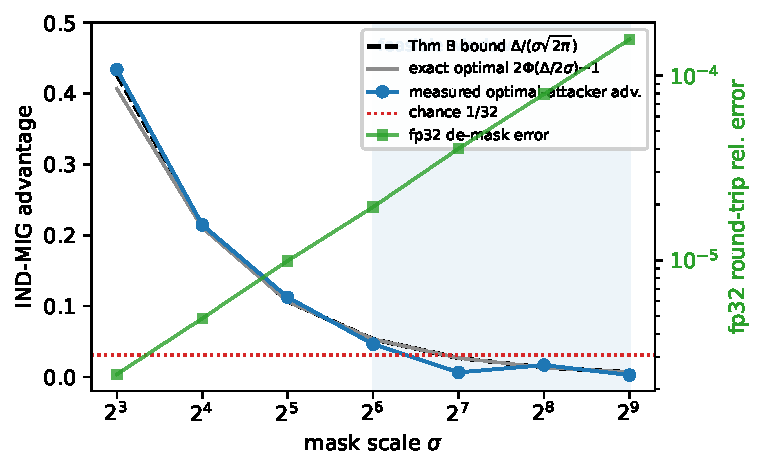
\includegraphics[width=\columnwidth]{figs/confidentiality_sweep.pdf}
\caption{RQ11. The measured optimal-attacker \textsc{IND-MIG} advantage (blue) tracks the Gaussian-mechanism bound of Theorem~\ref{thm:confidentiality} (dashed) and decays to the $1/32$ chance level, while the fp32 de-mask error (green, right axis) grows with $\sigma$ (Theorem~\ref{thm:precision}); the shaded band is the feasible window. Orthogonal protection is the $\sigma{=}0$ endpoint with advantage $1.0$.}
\label{fig:sweep}
\end{figure}

\textbf{The migration attacker is reduced to blind guessing.} Table~\ref{tab:ge} reports guessing entropy (mean rank of the true secret among $N{=}32$; $1$ = fully recovered, $(N{+}1)/2{=}16.5$ = chance). Orthogonal caches ($\sigma{=}0$) have guessing entropy $1.0$ on both models---the secret is always rank-1, i.e.\ zero residual uncertainty, consistent with Theorem~\ref{thm:impossible}. For any $\sigma\ge16$ the migration attacker's guessing entropy is at the chance level on both Qwen3-0.6B and Llama-3.2-1B: the affine mask leaves essentially the full $\log_2 N$ bits of uncertainty.

\begin{table}[t]
\centering
\caption{RQ11. Guessing entropy of the migration attacker (mean rank, $N{=}32$, chance $16.5$). Orthogonal ($\sigma{=}0$) fully recovers (GE $1.0$); affine leaves the secret at chance for $\sigma\ge16$.}
\label{tab:ge}
\begin{tabular}{@{}lcc@{}}
\toprule
$\sigma$ & Qwen3-0.6B & Llama-3.2-1B \\
\midrule
0 (orthogonal) & 1.0 & 1.0 \\
16 & 15.5 & 17.2 \\
64 & 15.6 & 17.4 \\
128 & 15.7 & 17.2 \\
512 & 15.8 & 17.2 \\
\bottomrule
\end{tabular}
\end{table}

\textbf{Adaptive attacks define the exact boundary.} Table~\ref{tab:adaptive} reports two attackers stronger than single-shot matching. Same-session known-plaintext recovers \emph{both} the basis (orthogonal Procrustes on cross-prompt differences, which cancel the mask) and the mask itself, stripping a held-out cache to residual $0.000$---so the affine mask, like the orthogonal basis, is broken under same-session KPA, and its protection is only for the migration attacker; under a refreshed nonce the recovered $(O,M)$ do not transfer (residual $\gg 1$). The averaging attacker, which needs the same secret cached many times under independent per-write masks, stays at chance through $10^5$ observations and reaches only top-1 $0.50$ (Qwen3) or chance (Llama) at $10^6$ observations: recovery requires $\Theta((\sigma\sqrt{d}/\lVert X\rVert)^2)$ identical re-cachings, an impractical capability. Together with the differencing attack (Table~\ref{tab:differencing}), these state the boundary precisely: the per-write nonce stops differencing, session refresh stops cross-session transfer, and same-session aligned known-plaintext is the designed non-goal.

\begin{table}[t]
\centering
\caption{RQ11. Adaptive attacks on the affine mask (std~128). KPA rows report strip residual (same-session $\to 0$ = broken; refreshed nonce $\gg 1$ = safe); averaging rows report top-1, needing $\ge 10^6$ identical re-cachings.}
\label{tab:adaptive}
\begin{tabular}{@{}lcc@{}}
\toprule
Attack & Qwen3-0.6B & Llama-3.2-1B \\
\midrule
KPA, same session & 0.000 & 0.000 \\
KPA, refreshed nonce & $\gg 1$ & $\gg 1$ \\
Averaging, $10^5$ obs. & 0.075 & 0.000 \\
Averaging, $10^6$ obs. & 0.500 & 0.025 \\
\bottomrule
\end{tabular}
\end{table}

\textbf{No plaintext is materialized, in use or at rest.} Finally, Table~\ref{tab:materialize} operationalizes Definition~\ref{def:inuse}. Encrypt-at-rest must decrypt a cache page to plaintext $V$ before attention, so an in-use memory snapshot yields plaintext and layer-0 V-inversion recovers every token (top-1 $1.000$, the RQ1 baseline). Orthogonal and affine \sys{} compute on the rotated coordinate $VO$ and never produce model-native plaintext anywhere in the memory hierarchy, so the same inversion on an in-use snapshot fails (top-1 $0.000$, the RQ2 cache-defense result). This is the property that distinguishes \sys{} from encryption even granting equal at-rest key handling.

\begin{table}[t]
\centering
\caption{RQ11. In-use materialization (Definition~\ref{def:inuse}). Layer-0 V-inversion top-1 on the tensor that attention actually consumes; only encrypt-at-rest exposes plaintext.}
\label{tab:materialize}
\begin{tabular}{@{}lcc@{}}
\toprule
Scheme & In-use tensor & V-inv \\
\midrule
AES-at-rest (decrypted) & plaintext $V$ & 1.000 \\
\sys{}, orth./affine & rotated $VO$ & \best{0.000} \\
\bottomrule
\end{tabular}
\end{table}

\textbf{Answer to RQ11:} The measured \textsc{IND-MIG} advantage tracks the Gaussian-mechanism bound of Theorem~\ref{thm:confidentiality} across $\sigma$ and decays to chance; the migration attacker's guessing entropy is at the $16.5$ chance level for $\sigma\ge16$ on both models (versus $1.0$ for orthogonal); same-session KPA is the precise non-goal while differencing, cross-session transfer, and averaging through $10^5$ observations are all defeated; and no plaintext K/V is materialized in use or at rest.

\subsection{Open Evaluation Gaps}

The Route~B experiments close the largest earlier gaps: the candidate audit now extends to $N=1000$ (RQ7) and confirms the advantage is flat in the candidate-set size, the differencing attack and its nonce fix are validated on real caches (RQ8), the head-to-head against encrypt-at-rest quantifies the materialization/throughput tradeoff (RQ9), and the PUF/FE assumptions are discharged in simulation (RQ10). Three gaps remain before submission. First, although the real-context PII benchmark covers public CC-News articles and real Enron emails, the secrets themselves are still seeded synthetically with exact scoring rather than mined from genuinely private records. Second, the PUF is simulated; RQ10 discharges the assumptions in software, but real FPGA traces are still needed to validate physical min-entropy, reliability, and helper-data leakage. Third, performance uses the unoptimized PyTorch wrapper: the orthogonal path composes with fused \texttt{scaled\_dot\_product\_attention} (Section~\ref{sec:discussion}), but fp16 FlashAttention and a fused affine de-masking cache-load kernel remain future work.

\section{Discussion}
\label{sec:discussion}

\subsection{Why binding helps, and why it is not enough}

Physical binding helps because it changes the coordinate system of the state that attackers observe. Plaintext cache attacks depend on alignment: inversion assumes that cached values live in the public projection basis, collision assumes that locally generated rows can be compared to leaked rows, and injection assumes that a standard model can interpret the stolen K/V history. Orthogonal \sys{} breaks these assumptions by storing K/V in a session-specific basis while preserving attention for the device that generated the basis.

The same experiments show why binding alone is not enough, and exactly which property a software-key obfuscator lacks that physical binding supplies. Our migration test makes the distinction concrete: a software obfuscator protects the cache only while its key stays secret, so an adversary who dumps the cache and the key from the same process recovers everything; \sys{} has no such key, so a copied cache plus the entire software stack stays bound to the originating device. This is the core reason to use a PUF, and it is a property of where the secret lives, not of avoiding decryption --- indeed our strongest confidentiality variant, affine masking, deliberately decrypts inside attention.

Binding is also not the same as confidentiality. An orthogonal map preserves not just row norms but every right-invariant statistic of the cache: the norms are only the diagonal of the Gram matrix $XX^\top$, which is itself preserved, as is the singular-value spectrum. Finite-candidate attackers can compare any of these without learning the session basis, and all three recover protected secrets at top-1 1.000. The design problem is therefore sharper than ``make the cache device-bound'': a protected cache must remove the whole basis-invariant class, which is what motivates the additive, non-orthogonal affine mask.

\subsection{Why fixed bases fail}

A natural conjecture is that a PUF-derived basis is secure because the PUF root is physically unclonable. Our profiling results reject that conjecture for fixed sessions. If an adversary obtains aligned plaintext/protected pairs from the same session, the adversary does not need to clone the PUF; the adversary can learn the induced orthogonal map directly. This distinction reframes the design problem: the PUF root provides device binding, but session refresh provides profiling resistance.

The invariant-class result rejects a second conjecture: that any unknown orthogonal basis is sufficient for cache-only confidentiality. Norm, Gram-matrix, and singular-spectrum matchers each recover protected finite secrets with top-1 accuracy 1.000 on Qwen3-0.6B and Llama-3.2-1B. This is why we treat orthogonal \sys{} as a binding baseline and affine masking as the current confidentiality-oriented redesign.

\subsection{Why affine masking is the current redesign candidate}

Unit-normalizing exported cache rows blocks the norm attack in our prototype, but it requires a trusted sidecar for the original norms. That sidecar weakens the system story: if the deployment already has trusted storage for per-row metadata, reviewers can ask why the KV cache itself is not stored there. Affine masking avoids that objection. The mask is not stored as content metadata; the device regenerates it from the PUF root, session nonce, layer, head, and position.

Affine masking is not free. It changes the orthogonal-only property that attention can operate directly on protected coordinates; the legitimate path now regenerates and subtracts masks inside attention. It also introduces cancellation risk, visible in the Qwen3 fp32 sanity gap increasing from roughly $3\times10^{-5}$ for the orthogonal path to $4.90\times10^{-4}$ at mask std128, and it roughly doubles decode overhead. The mask strength is a controllable tradeoff: sweeping it shows the strongest invariant (Gram) attack falling from $0.975$ at std~4 to near the $1/32$ chance level by std~64--128, while the fp32 error grows monotonically, so std~128 is the knee rather than a tuned constant. The security gain is correspondingly larger: it removes the whole invariant class (Qwen3 Gram/spectrum/norm top-1 to $0.033/0.033/0.050$). These numbers make affine masking the best current direction, not a completed production design.

\subsection{Precision is a systems requirement}

The fp32 results show exact equivalence, whereas bf16 long-decode experiments expose early divergence on two prompts. This result does not invalidate the algebraic construction; it shows that protected-coordinate arithmetic can redistribute channel magnitudes and thereby change low-precision rounding trajectories. For deployment, the relevant question is not whether the identity holds in real arithmetic, but whether the inference stack preserves enough precision for the identity to remain behaviorally stable. Affine masking raises this requirement further because large masks must be subtracted before attention. We therefore treat fp32 attention activations, fp32 cache storage, stochastic rounding, or masking families optimized for quantized inference as implementation choices rather than optional refinements.

Rather than treating cache protection as a storage-layer encryption problem, we argue that LLM serving systems should treat persistent attention state as session-bound computation state. This prescription changes which secrets must survive compromise: copied tensors should not be enough to reconstruct or replay the original context.

\subsection{Compatibility with fused attention kernels}

Because the cache-migration surface is created by optimized serving systems --- paged attention and KV offloading --- a defense must eventually run inside their fused kernels rather than in eager attention. The orthogonal path composes cleanly with the standard fused entry point: the rotations are linear maps applied to $q$, $k$, and $v$ \emph{around} attention, so routing the rotated tensors through \texttt{scaled\_dot\_product\_attention} reproduces the plain logits to within $4\times10^{-5}$, and the $O_k$/$O_v$ multiplications fold naturally into the QKV and output projections. In fp32 this dispatches to the math/memory-efficient backend; fp16 FlashAttention additionally requires the precision care discussed below. The affine-mask path is the harder case, because the mask must be subtracted between the cache read and the QK/AV products. We implemented a fused Triton flash-decoding kernel that regenerates the PUF mask in-register via the same counter-based Philox RNG as the write path and subtracts it in the SRAM epilogue of the KV load, so de-masking adds no HBM traffic and no separate pass (RQ12, Table~\ref{tab:fused-kernel}). A split-K design (grid $(B,H_q,n_{\text{splits}})$ plus a log-sum-exp reduction) lifts SM occupancy and eliminates the long-context regression a naive single-program-per-head kernel suffers. The fused output is token-identical to the eager de-mask path on both Qwen3-0.6B and Llama-3.2-1B and is $4$--$5$ percentage points cheaper in decode overhead ($\approx{-}29\%$ vs.\ plain, against $\approx{-}33\%$ for eager). The precision concern is also milder than the bf16 result suggests: fp16, the precision FlashAttention typically uses, diverges on only $14.1\%$ of continuations for the fused affine path versus $20.3\%$ for both orthogonal and eager-affine (all at 64 prompts and 64 tokens, fp32 cache; the shorter 32-token diagnostic in RQ3 gives $15.6\%$/$56.25\%$ for fp16/bf16 respectively---the rate grows with decode length but the ordering is stable), because fp16's larger mantissa resolves the rotated channel magnitudes and the fused kernel keeps the entire de-mask in fp32. Paged and flash-attention integration of the fused kernel remains engineering work.

\subsection{Scope: where physical binding is the right tool}

\sys{} is not a drop-in replacement for confidential-computing enclaves. Its niche is edge and on-premise inference where a trusted execution environment is unavailable or unattested but the device has a usable PUF/root-of-trust, and where the realistic threat is post-compromise migration of persistent cache state rather than a live attacker inside the running enclave. In that setting the alternatives are weaker: software-key obfuscation migrates with the cache, and full KV encryption requires a device-bound key whose lifecycle must itself be solved. Where a strong attested TEE is available, it subsumes much of this; \sys{} targets the large deployment surface where it is not.

\subsection{Limitations}

The current prototype has five primary limitations. First, orthogonal \sys{} is not a complete confidentiality mechanism because the full basis-invariant class --- norm, Gram, and spectrum matching --- recovers protected secrets with top-1 accuracy 1.000. Second, affine masking removes that class and is now utility-validated (fp32-exact on perplexity, HellaSwag, MMLU, and long decoding) with a fused split-K de-masking kernel validated at $\approx 29\%$ decode overhead (RQ12), but it remains fp32-only and the kernel targets contiguous-cache decode rather than paged/flash serving. Third, the square-projection inversion attack that gives the dramatic top-1 1.000 token-recovery baseline is specific to Qwen3-0.6B; on the other families we rely on injection and finite-candidate matching, which generalize but are less visually striking, so the cross-model leakage story rests on those rather than on inversion. Fourth, the PUF is simulated, so the current work validates the software interface and noise model but not physical reliability, uniqueness, or helper-data leakage. Fifth, the fused kernel is benchmarked on the decode path in isolation; full integration with paged-attention and flash-attention serving stacks (including prefill fusion and bf16/fp16 policies) remains engineering work.

These limitations define the next mechanism rather than invalidate the direction. Non-square projection attacks can use injection, finite-candidate matching, and task-level leakage metrics rather than square V-inversion. Physical PUF traces can replace the simulator root while preserving the HMAC context derivation. Serving benchmarks can measure the cost of fused rotation and mask-subtraction kernels under bf16, fp32, and fp32-cache policies.

\section{Related Work}
\label{sec:related}

\textbf{KV-cache privacy attacks and defenses.} Shadow in the Cache identifies inversion, collision, and injection attacks against plaintext KV-caches and proposes KV-Cloak as a software-secret obfuscation defense \cite{shadow_cache}. Our work builds on that threat surface but changes the trust boundary: \sys{} binds the cache representation to a physical session basis rather than to exportable software matrices. The broader class of microarchitectural cache side-channel attacks, such as \textsc{Flush+Reload}~\cite{flush_reload}, motivates treating leaked cache state as an exploitable observation surface rather than inert storage.

\textbf{Efficient LLM serving.} KV-cache systems, paged attention, and cache offloading improve throughput by externalizing persistent inference state. This performance optimization inadvertently creates the cache-at-rest and cache-migration surface studied in this paper. Orthogonal \sys{} preserves the reuse semantics of the cache instead of encrypting and decrypting it around every attention operation; affine masking preserves reuse but requires mask subtraction inside attention. Systems such as PagedAttention/vLLM~\cite{pagedattention} and offloading engines like FlexGen~\cite{flexgen} externalize and migrate this persistent state for throughput, which is precisely what enlarges the cache-migration attack surface.

\textbf{Hardware roots of trust and PUFs.} PUFs have been used for device authentication and key derivation. \sys{} uses the PUF root differently: the PUF determines the coordinate system and affine masks in which attention state is stored. This makes PUF security not only an identity property but also a state-interpretation property. Our construction builds on classic silicon PUFs~\cite{gassend_silicon} and PUF-based key generation~\cite{suh_devadas_puf}, together with fuzzy extractors~\cite{dodis_fuzzy} for stable root reconstruction from noisy responses.

\textbf{Confidential inference and TEEs.} Trusted execution environments and confidential accelerators protect runtime secrets, but high-throughput LLM serving often externalizes large KV state for memory efficiency. \sys{} complements these approaches by reducing what must remain secret after a cache leaves the protected runtime: copied cache tensors remain bound to the originating session basis or affine mask. GPU TEEs such as Graviton~\cite{graviton} protect runtime secrets inside an isolated execution context, whereas \sys{} targets the complementary problem of state that has already left that context.

\section{Conclusion}
\label{sec:conclusion}

We presented \sys{}, a PUF-bound KV-cache design study that separates device/session binding from full cache confidentiality. Orthogonal attention bases store K/V tensors in a device-session coordinate system while preserving attention equivalence for the legitimate device; on Qwen3-0.6B, this reduces attacker-view V-inversion from 1.000 to 0.000 and exact PII keyword leakage from 52.2\% to 0.0\%, and a migration test shows that a copied cache plus the full software stack stays uninterpretable on a device with a different PUF root, where a software-key obfuscator would not. The same orthogonal design fails against the whole basis-invariant class: norm, Gram-matrix, and singular-spectrum matching each recover protected secrets with top-1 accuracy 1.000 on Qwen3-0.6B and Llama-3.2-1B. A no-sidecar affine-mask redesign removes the class, driving every invariant attack to the $1/32$ chance level while staying fp32-exact on perplexity, HellaSwag, MMLU, and long decoding, at the cost of an in-attention de-masking step whose fused split-K Triton kernel adds $\approx 14$ percentage points of decode overhead over the orthogonal path ($-29\%$ versus $-15\%$ from plain). These results refine the core insight: the value of physical binding is non-migratability with no extractable key, and a confidential design must additionally remove the basis-invariant statistics that remain comparable after migration.


\IfFileExists{IEEEtran.bst}{\bibliographystyle{IEEEtran}}{\bibliographystyle{plain}}
\bibliography{reference}

\end{document}
